\chapter{RESULTS AND DISCUSSION}
\label{ch:results}

% This is Chapter 4 - Results and Discussion
% Present and discuss your experimental results

\section{Training Results}
This section will present the training results for all three YOLOv8 variants, trained on the Bundesliga Shootout Dataset for player and ball detection. Each model was trained using the identical hyperparameters described on the previous chapter. Training was set for 50 epochs, but early-stopping was implemented to prevent any models from training longer than necessary. The best performing checkpoint per model is used for all reported metrics, saved at the epoch with the highest validation mAP@0.5.
\subsection{Training Convergence}
Figure 4.1 depicts a clear picture of the evolution of training box loss, validation mAP@0.5, precision, and recall across 50 epochs for each model. Validation loss tracked training loss throughout the epochs, meaning we do not see any signs of overfitting. Training box loss decreased from approximately 2.3 in epoch 1 to below 1.8 for all models by epoch 50, with YOLOv8m achieving the lowest final training loss (1.48) due to its greater model capacity.

\begin{figure}[H]
    \centering
    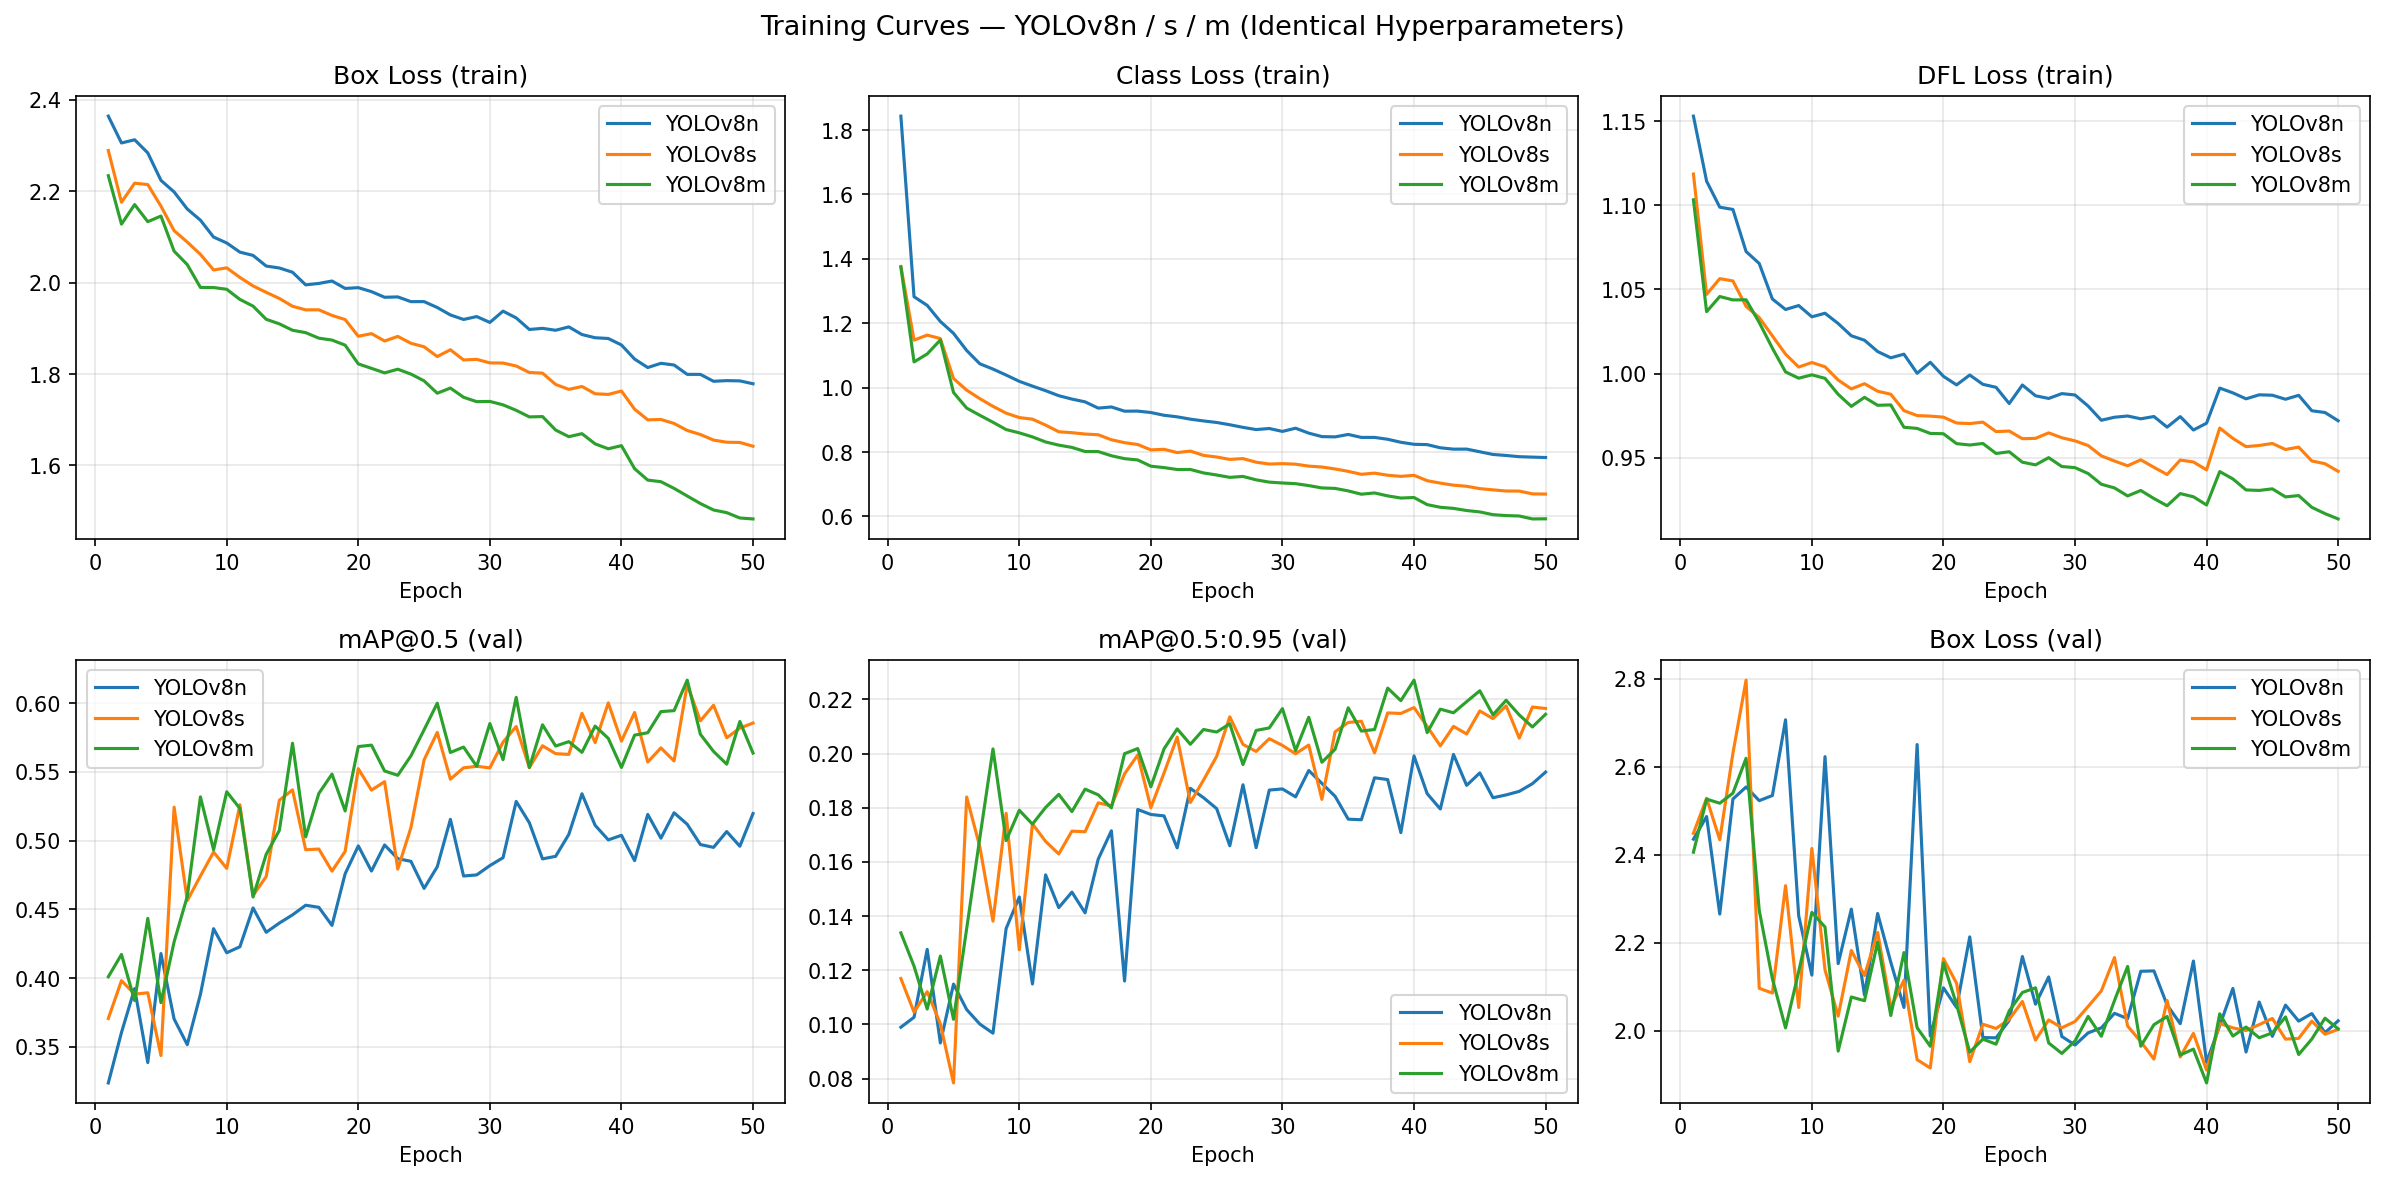
\includegraphics[width=1\textwidth]{figures/training_curves.png}
    \caption{Training curves for all three models during 50 epochs}
    \label{fig:training_curves}
\end{figure}

The mAP@0.5 curves show that initial improvement for all three models was rapid, especially during the first 10 epochs. The best performance was achieved around the 40th epoch for all models, after which we notice plateues or minor fluctuations. This pattern is usual for small datasets due to the model exhausting learning material relatively quickly.

\subsection{Detection Metrics}
Table 4.1 reports the validation metrics for each model’s best epoch. The small and medium models achieve almost identical overall mAP@0.5 scores of 0.613 and 0.617 respectively, as the difference of 0.004 is not statistically meaningful in a 38 image validation set. The nano model performs noticably worse in all metrics, clearly showing the limitations of its smaller capacity of 3M parameters for this detection task.

\begin{table}[H]
\centering
\label{tab:training_results}
\begin{tabular}{lccccc}
\hline
\textbf{Model} & \textbf{Precision} & \textbf{Recall} & \textbf{mAP@0.5} & \textbf{mAP@0.5:0.95} & \textbf{Train Time (min)} \\
\hline
YOLOv8n & 0.736 & 0.528 & 0.534 & 0.191 & 11.8 \\
YOLOv8s & 0.775 & 0.613 & 0.613 & 0.216 & 33.5 \\
YOLOv8m & 0.698 & 0.632 & 0.617 & 0.223 & 50.4 \\
\hline
\end{tabular}
\caption{Best-epoch validation metrics for all three model variants}
\end{table}

An interesting distinction between the  YOLOv8s and  YOLOv8m medium models lies on the precision-recall tradeoff. The small model achieves higher precision, while medium model achieves higher recall. This indicates that the medium model is more aggressive with its detections and therefore generates more true positives. The small model is pickier and better calibrated for the size of this dataset. 

\subsection{Class Detection Performance}
Breaking down the class detection performance reveals a very important finding in our training evaluation. From the figures in Table 4.2 we can see that while player detection is strong across all models, the ball detection remains substantially weaker. This weakness lines up with other studies of the same domain which we covered in the second chapter of this thesis. This weakness, however,  also proves to be the biggest difference maker across model sizes. 

\begin{table}[H]
\centering
\label{tab:perclass_ap}
\begin{tabular}{lcc}
\toprule
\textbf{Model} & \textbf{Ball AP} & \textbf{Player AP} \\
\midrule
YOLOv8n & 0.097 & 0.906 \\
YOLOv8s & 0.270 & 0.927 \\
YOLOv8m & 0.167 & 0.940 \\
\bottomrule
\end{tabular}
\caption{Per-class average precision (AP) for all three model variants}
\end{table}

The YOLOv8n model continues to show the limitations of its small parameter size, with the lowest metrics across both classes. Between the small and medium models, we notice more interesting differences. While the medium model performs slightly better at player detection, the small model shows distinctly better ball detection performance. This non-linear relationship between model size and detection accuracy shows a weakness of our study, which is the dataset size. With the small number of ball instances in the validation set, the larger model struggles to generalise to this underrepresented class.

\subsection{Precision-Recall Curves}
Below are the resulting precision-recall curves for each of our trained models. In all cases, a similar picture as seen above shows. The player detection curve shows strong performance by occupying the upper-right region of the plot, while the ball curve is substantially lower and more irregular. 

\begin{figure}[H]
    \centering
    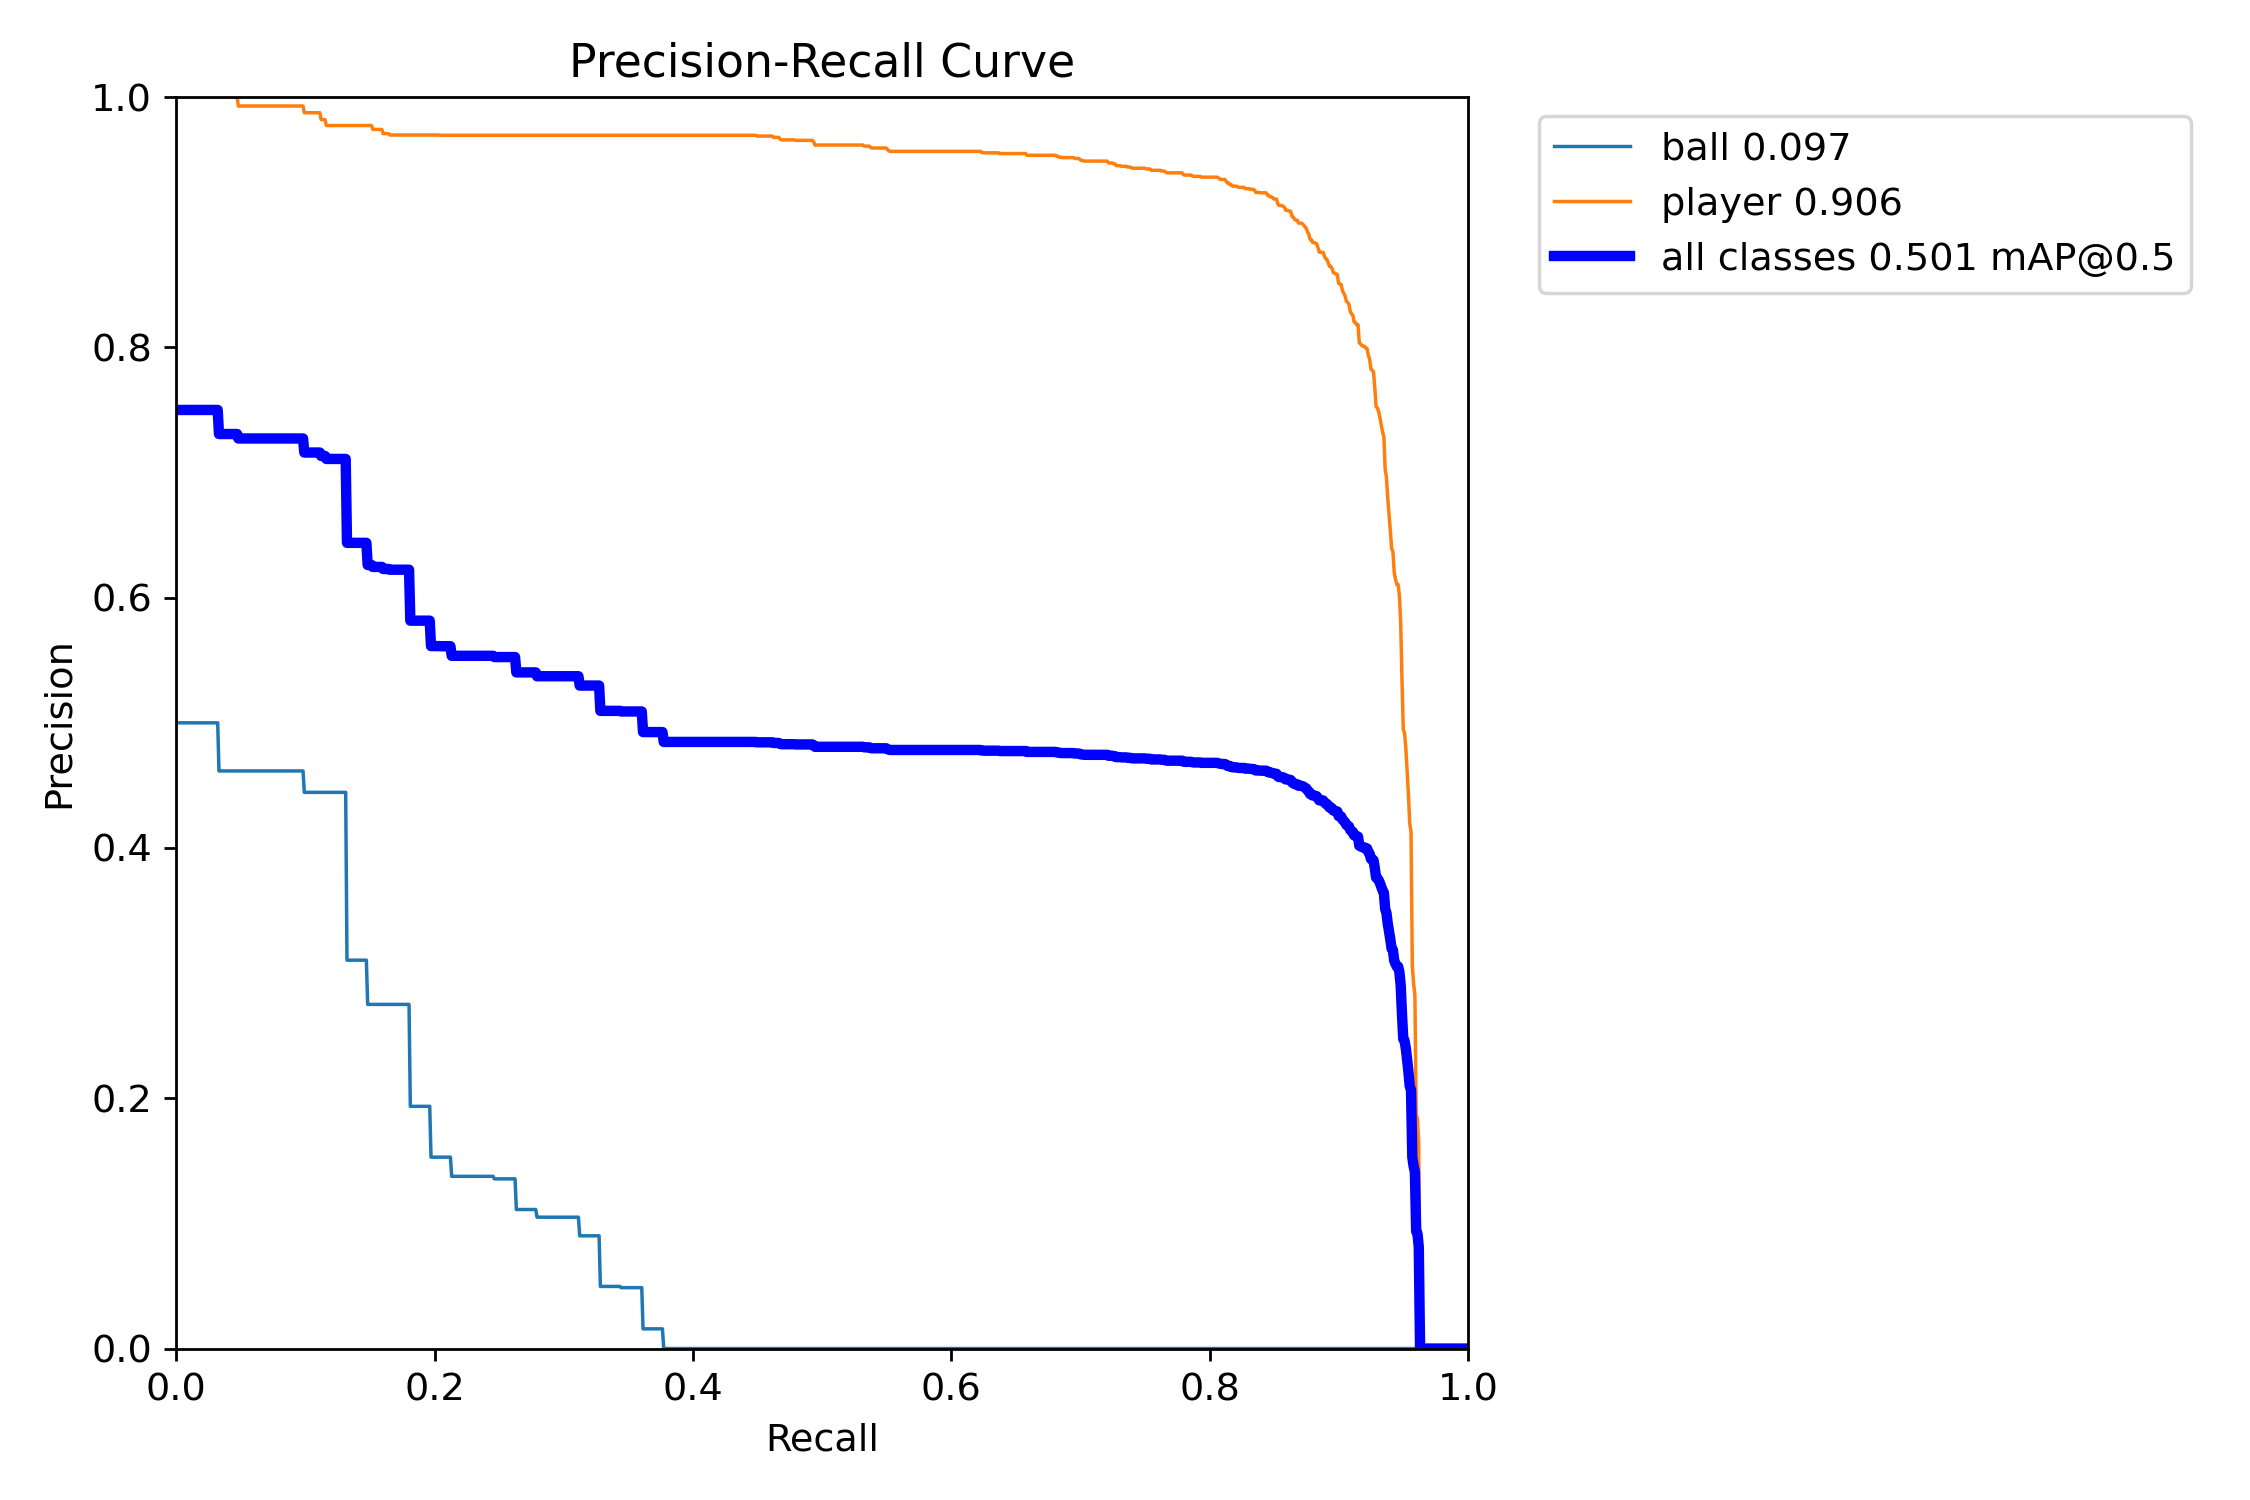
\includegraphics[width=1\textwidth]{figures/BoxPR_curve_n.png}
    \caption{Precision-Recall curve for the YOLOv8n model}
    \label{fig:P-R_nano}
\end{figure}
\noindent\rule{\textwidth}{0.4pt}
\begin{figure}[H]
    \centering
    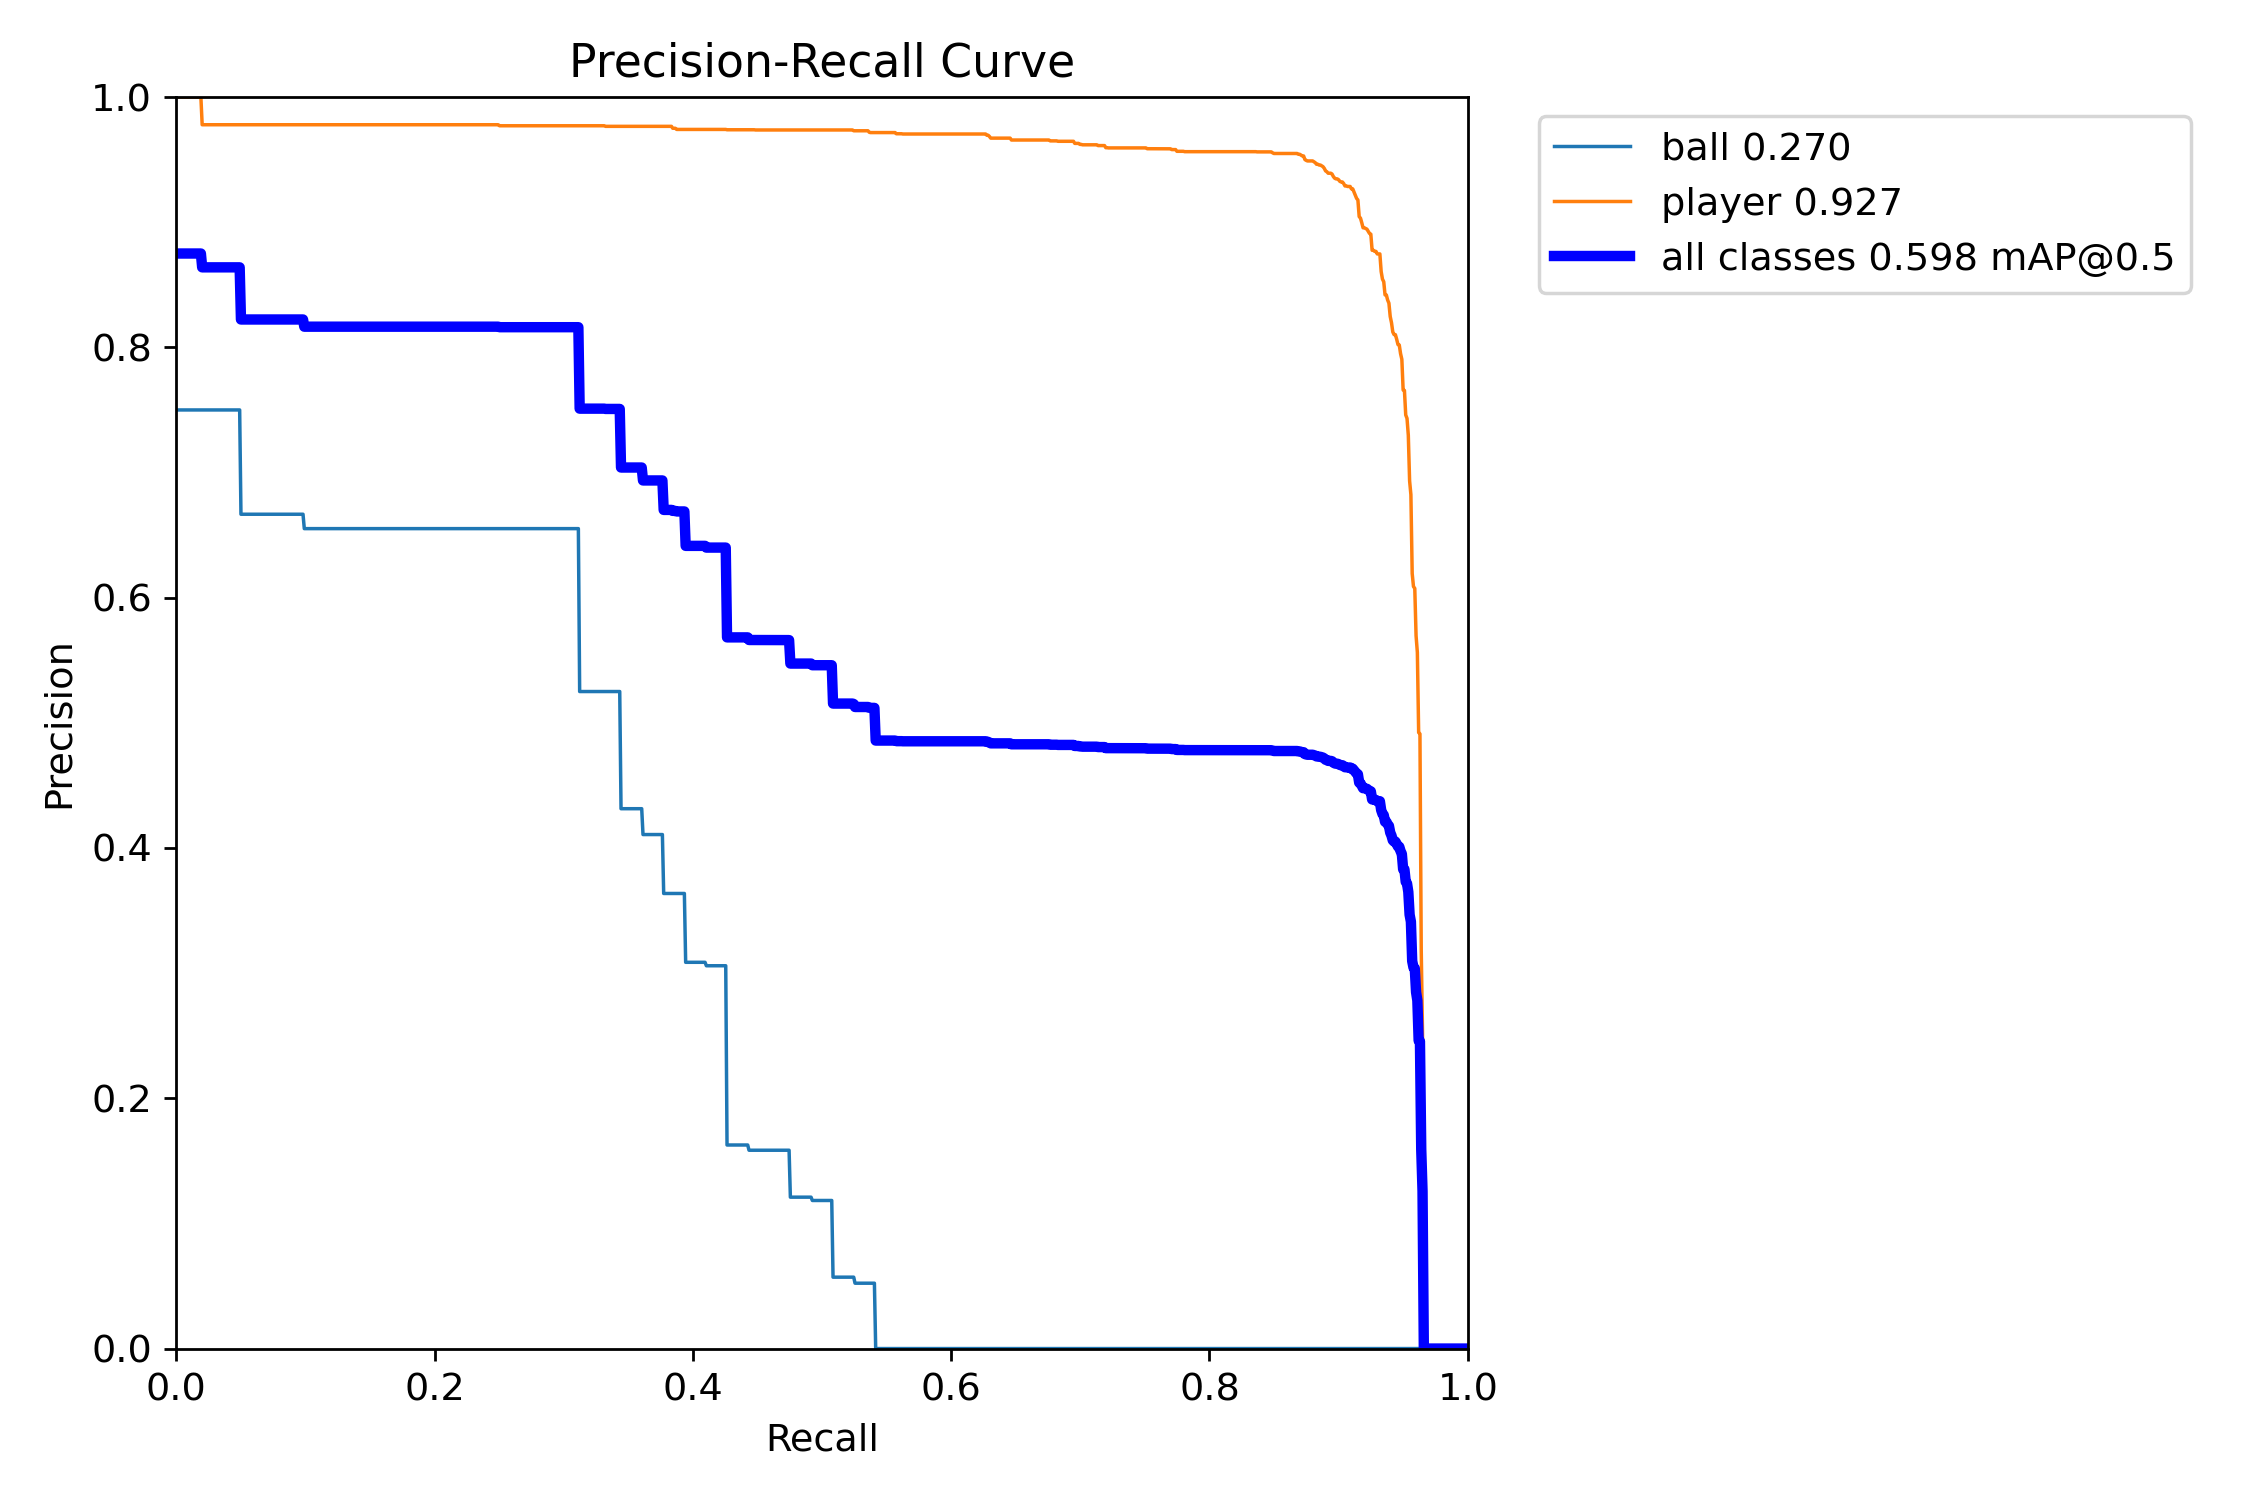
\includegraphics[width=1\textwidth]{figures/BoxPR_curve_s.png}
    \caption{Precision-Recall curve for the YOLOv8s model}
    \label{fig:P-R_small}
\end{figure}
\noindent\rule{\textwidth}{0.4pt}
\begin{figure}[H]
    \centering
    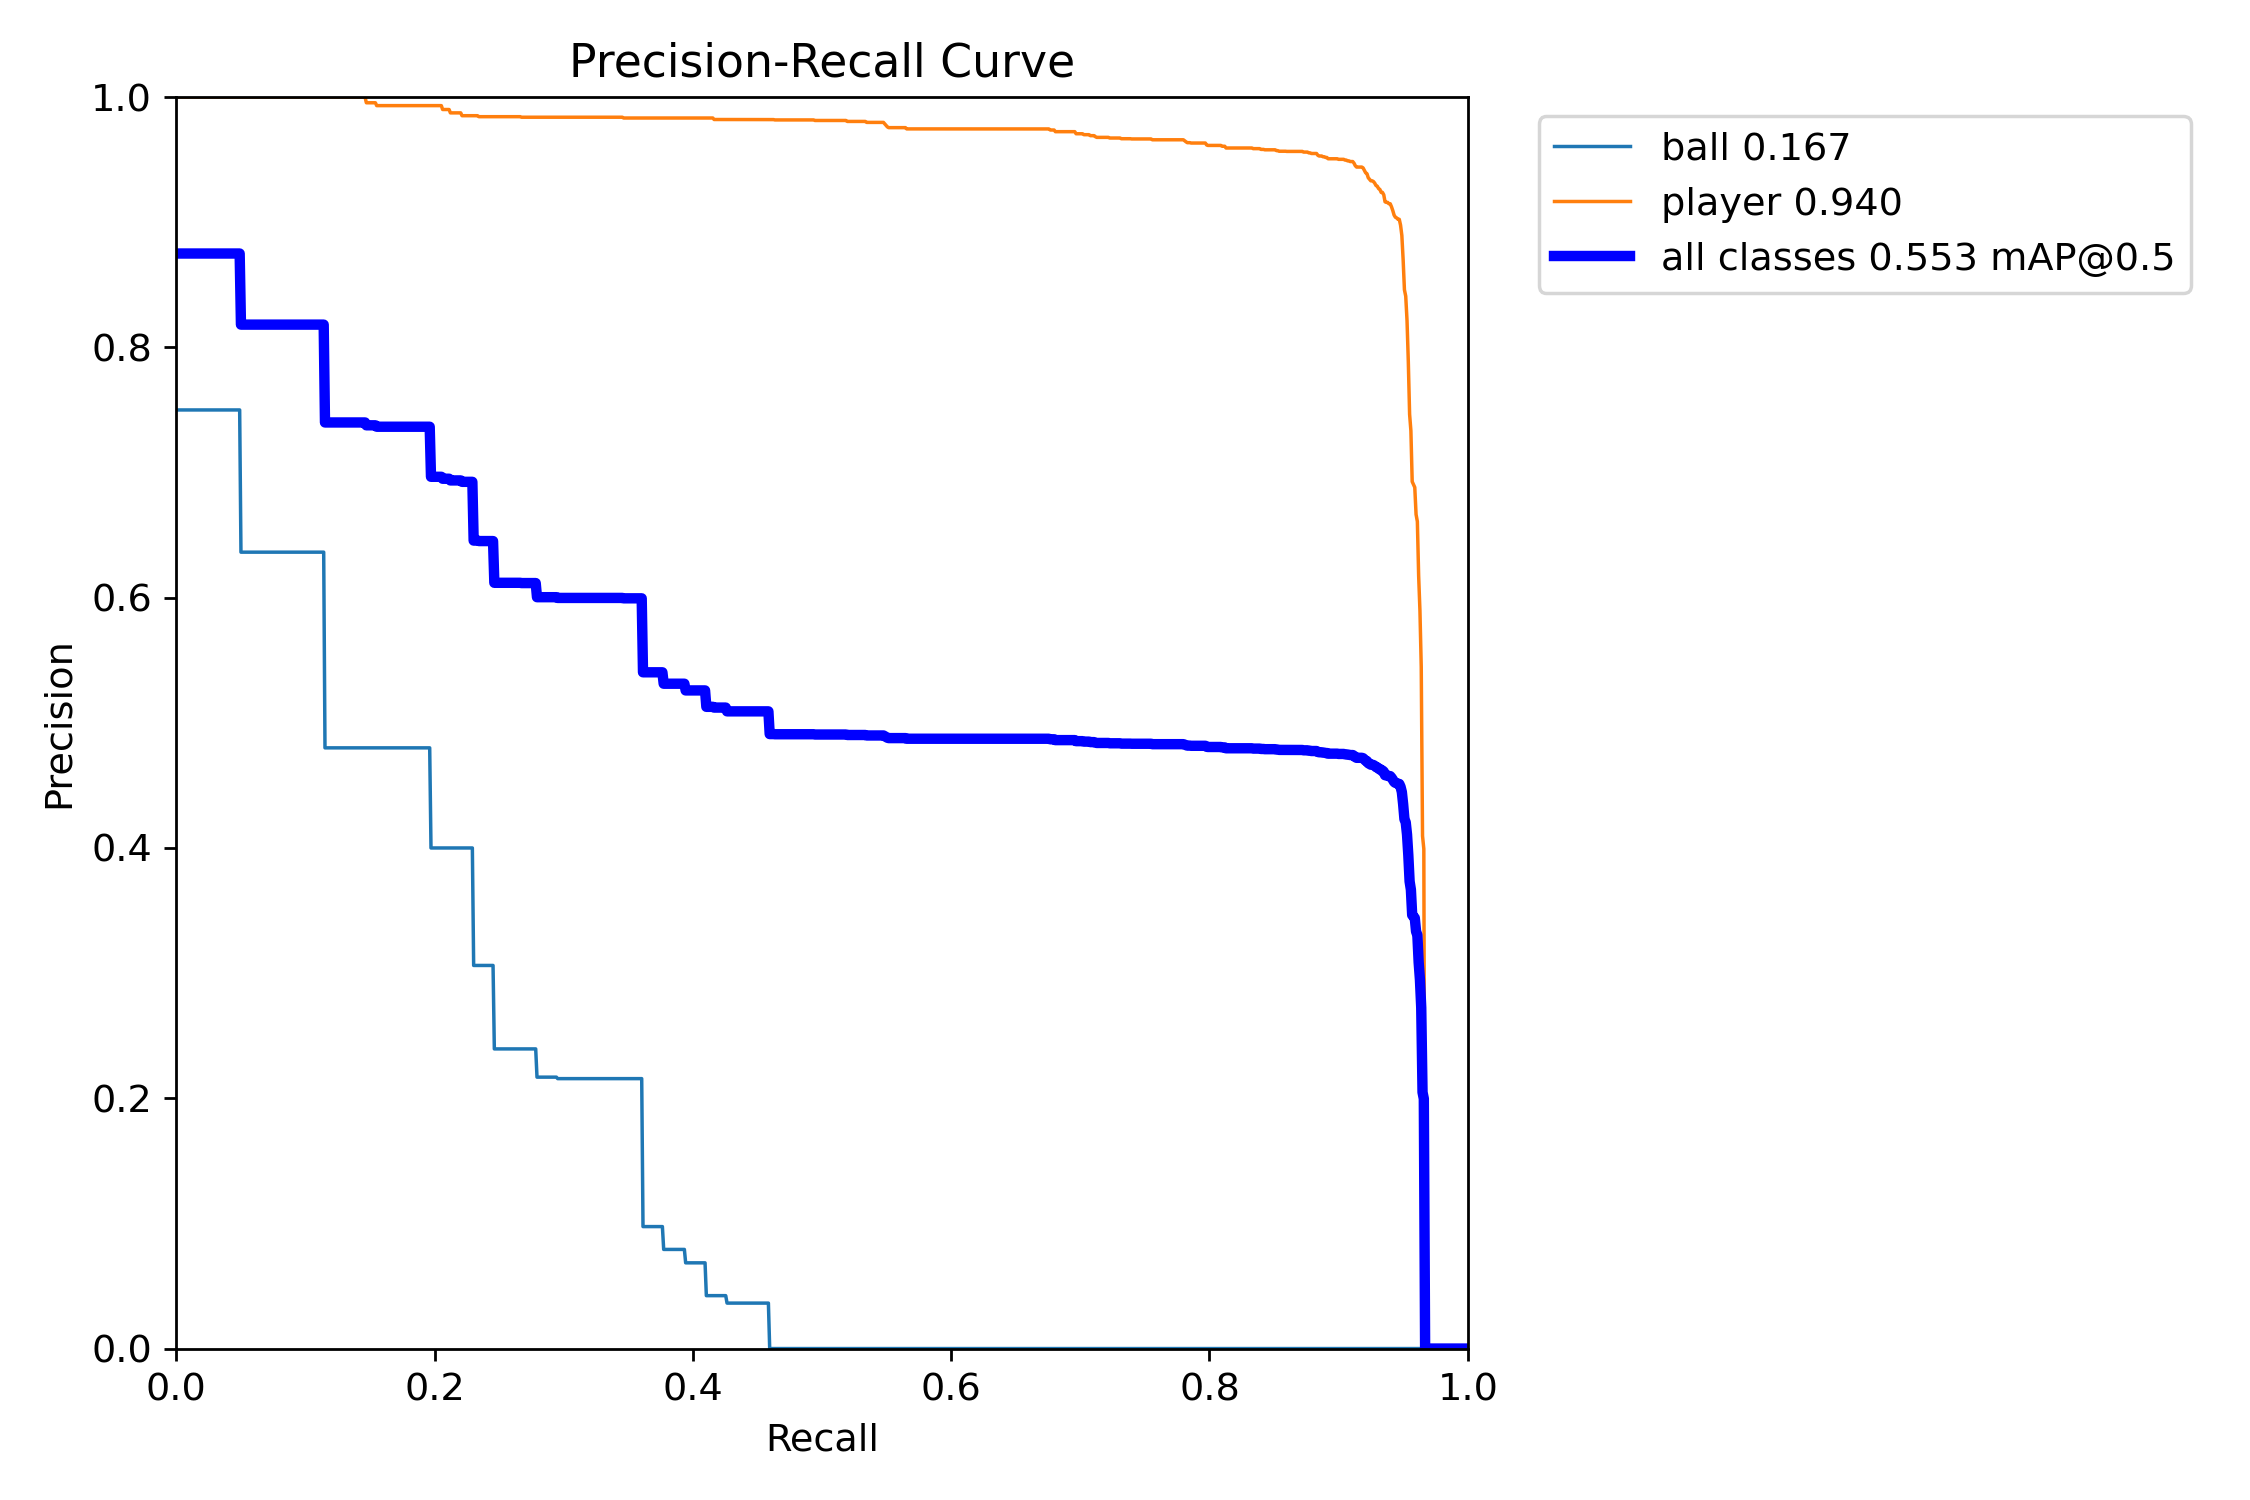
\includegraphics[width=1\textwidth]{figures/BoxPR_curve_m.png}
    \caption{Precision-Recall curve for the YOLOv8m model}
    \label{fig:P-R_medium}
\end{figure}

\subsection{Confusion Matrices}
Figures 4.5, 4.6 and 4.7 present the confusion matrices for each model evaluated on the validation set. These results reinforce the class-level AP findings. Player detections are accurate across all models. A significant error pattern is found from player detections being assigned to the background class. This shows missed detection rather than confusion between object classes.

Ball detections remain, as seen earlier, particularly difficult. The YOLOv8 model performs especially poorly, with only 11 true ball instances being correctly detected and 48 missed as background. This comes as a limitation of the image resolution picked for our pipeline, as a 640x640 image proves to be too blurry for small objects such as the ball to be properly differentiated from the background. YOLOv8s improves on the nano model to 22 correct detections and 39 missed, representing the best ball recall of the three models.

\begin{figure}[H]
    \centering
    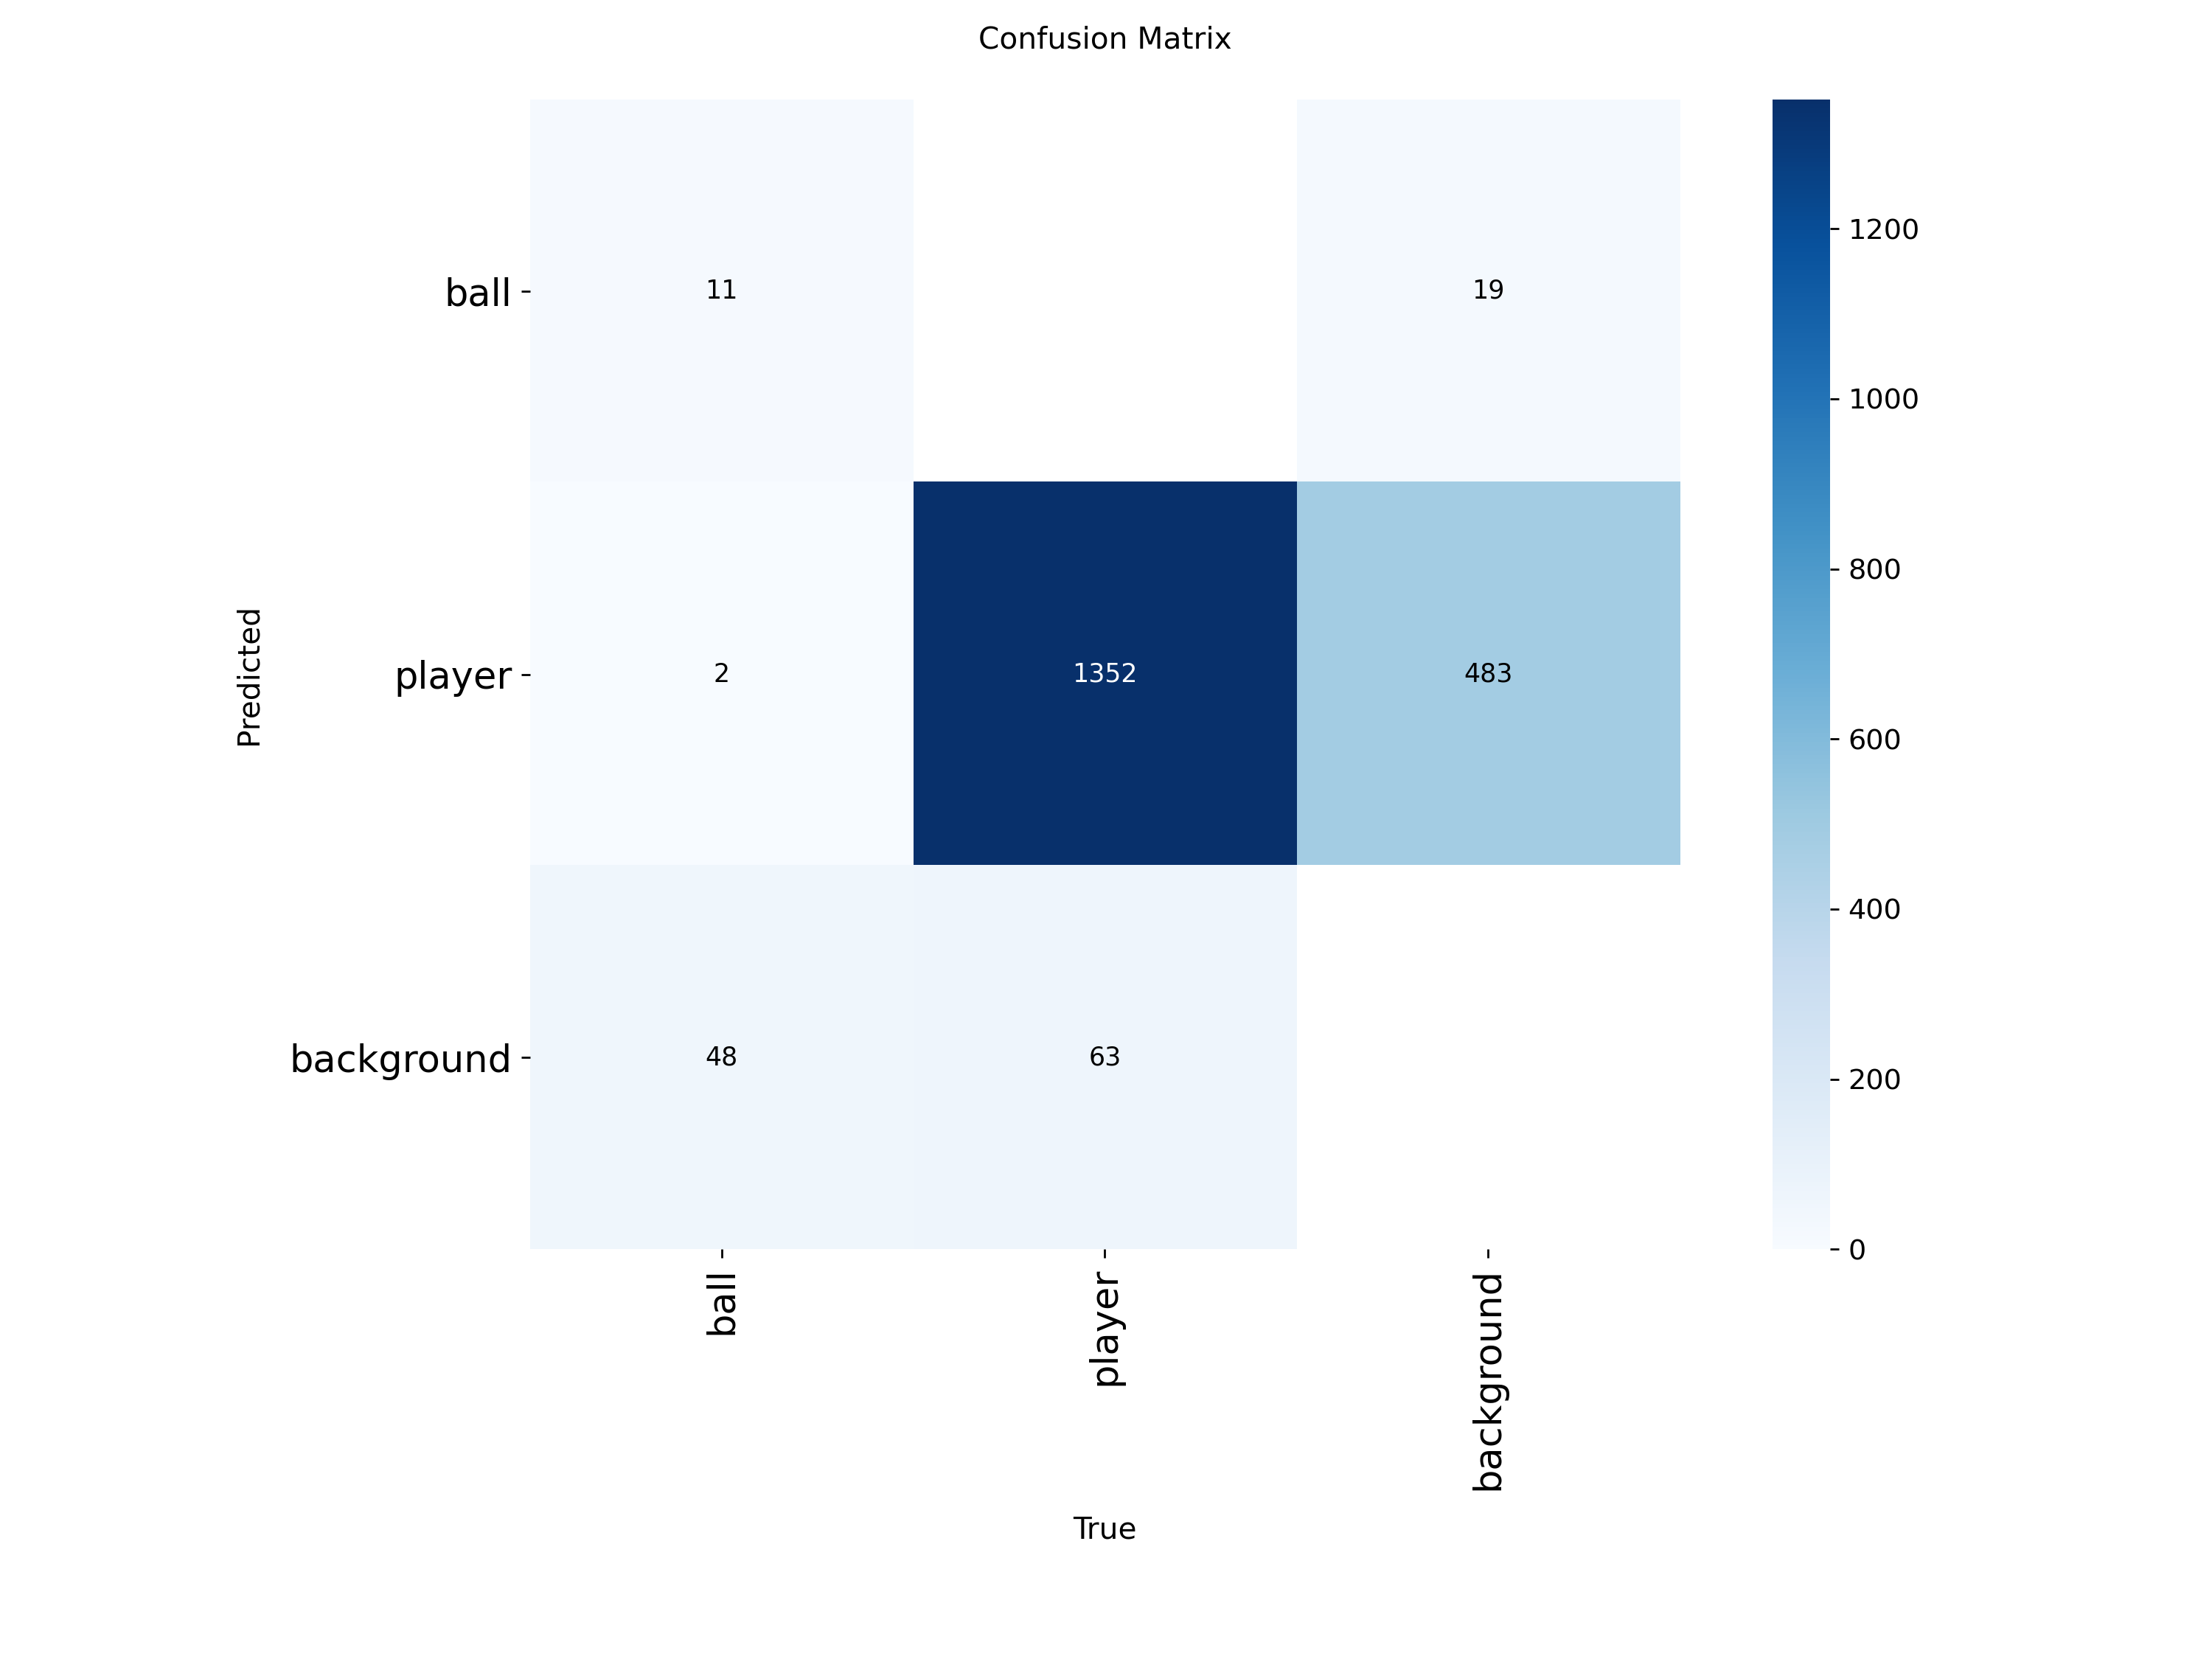
\includegraphics[width=0.8\textwidth]{figures/confusion_matrix_n.png}
    \caption{Confusion matrix for the YOLOv8n model}
    \label{fig:cm_n}
\end{figure}
\noindent\rule{\textwidth}{0.4pt}
\begin{figure}[H]
    \centering
    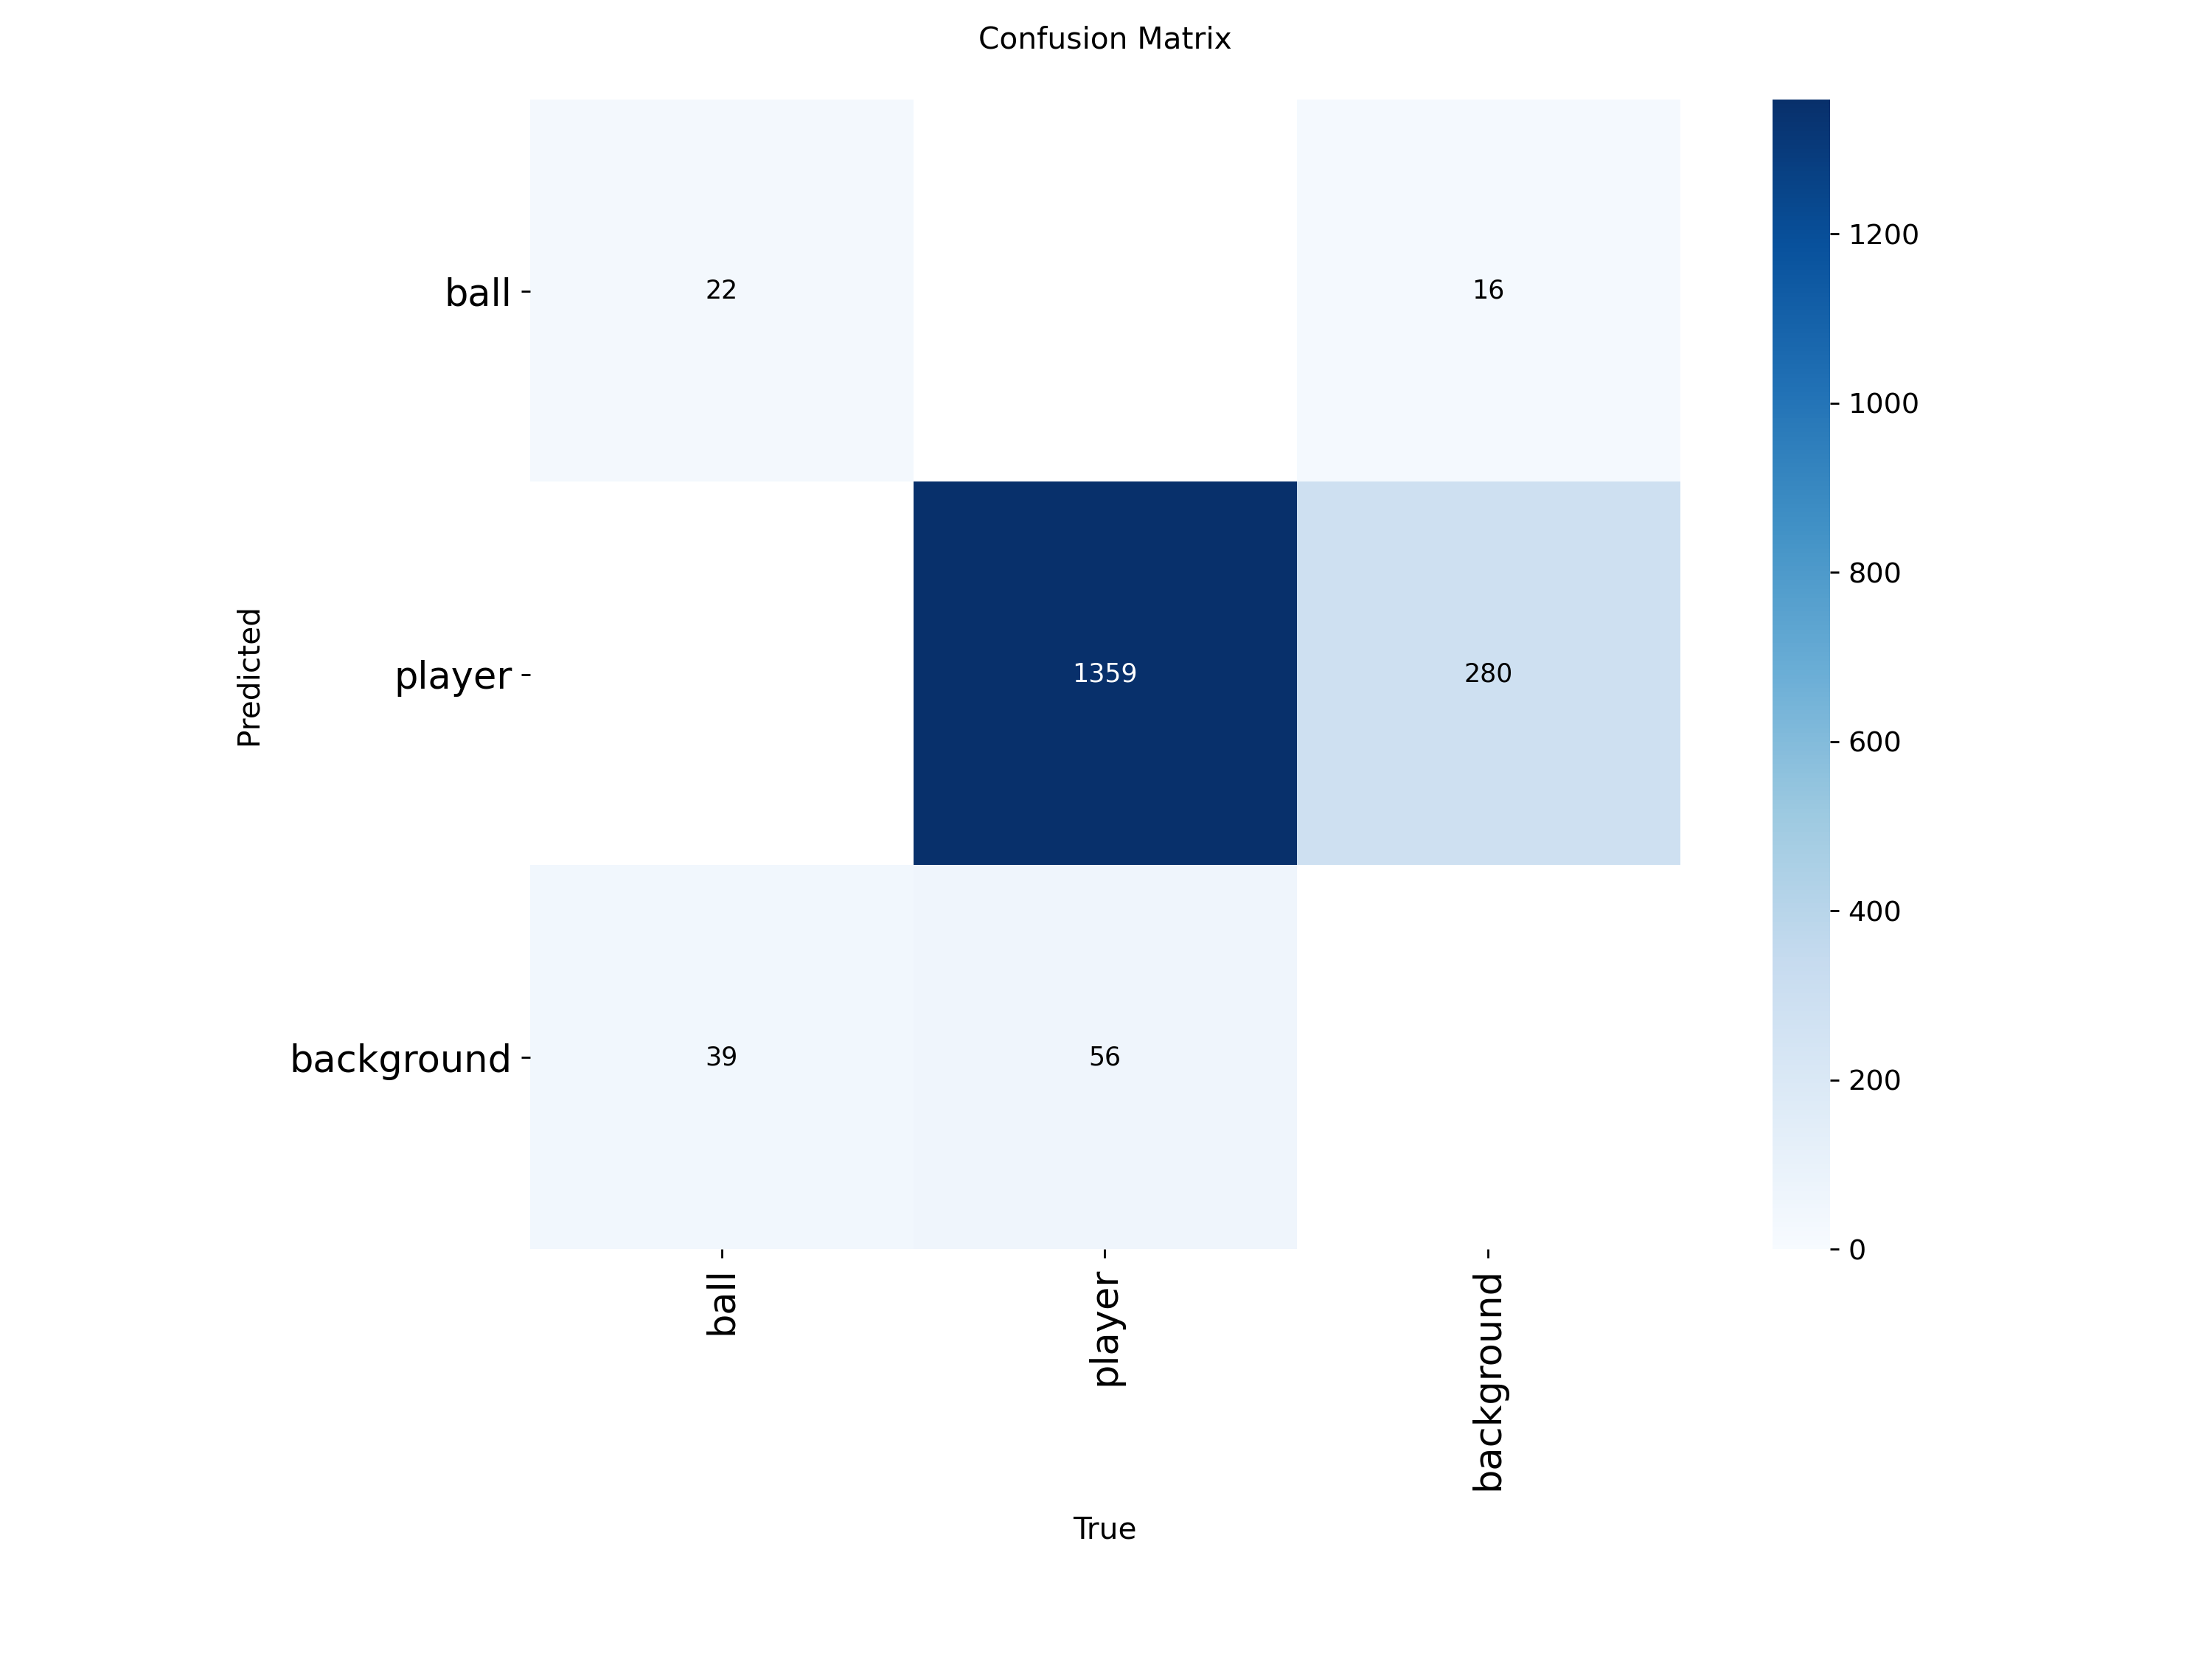
\includegraphics[width=0.8\textwidth]{figures/confusion_matrix_s.png}
    \caption{Confusion matrix for the YOLOv8s model}
    \label{fig:cm_s}
\end{figure}
\begin{figure}[H]
    \centering
    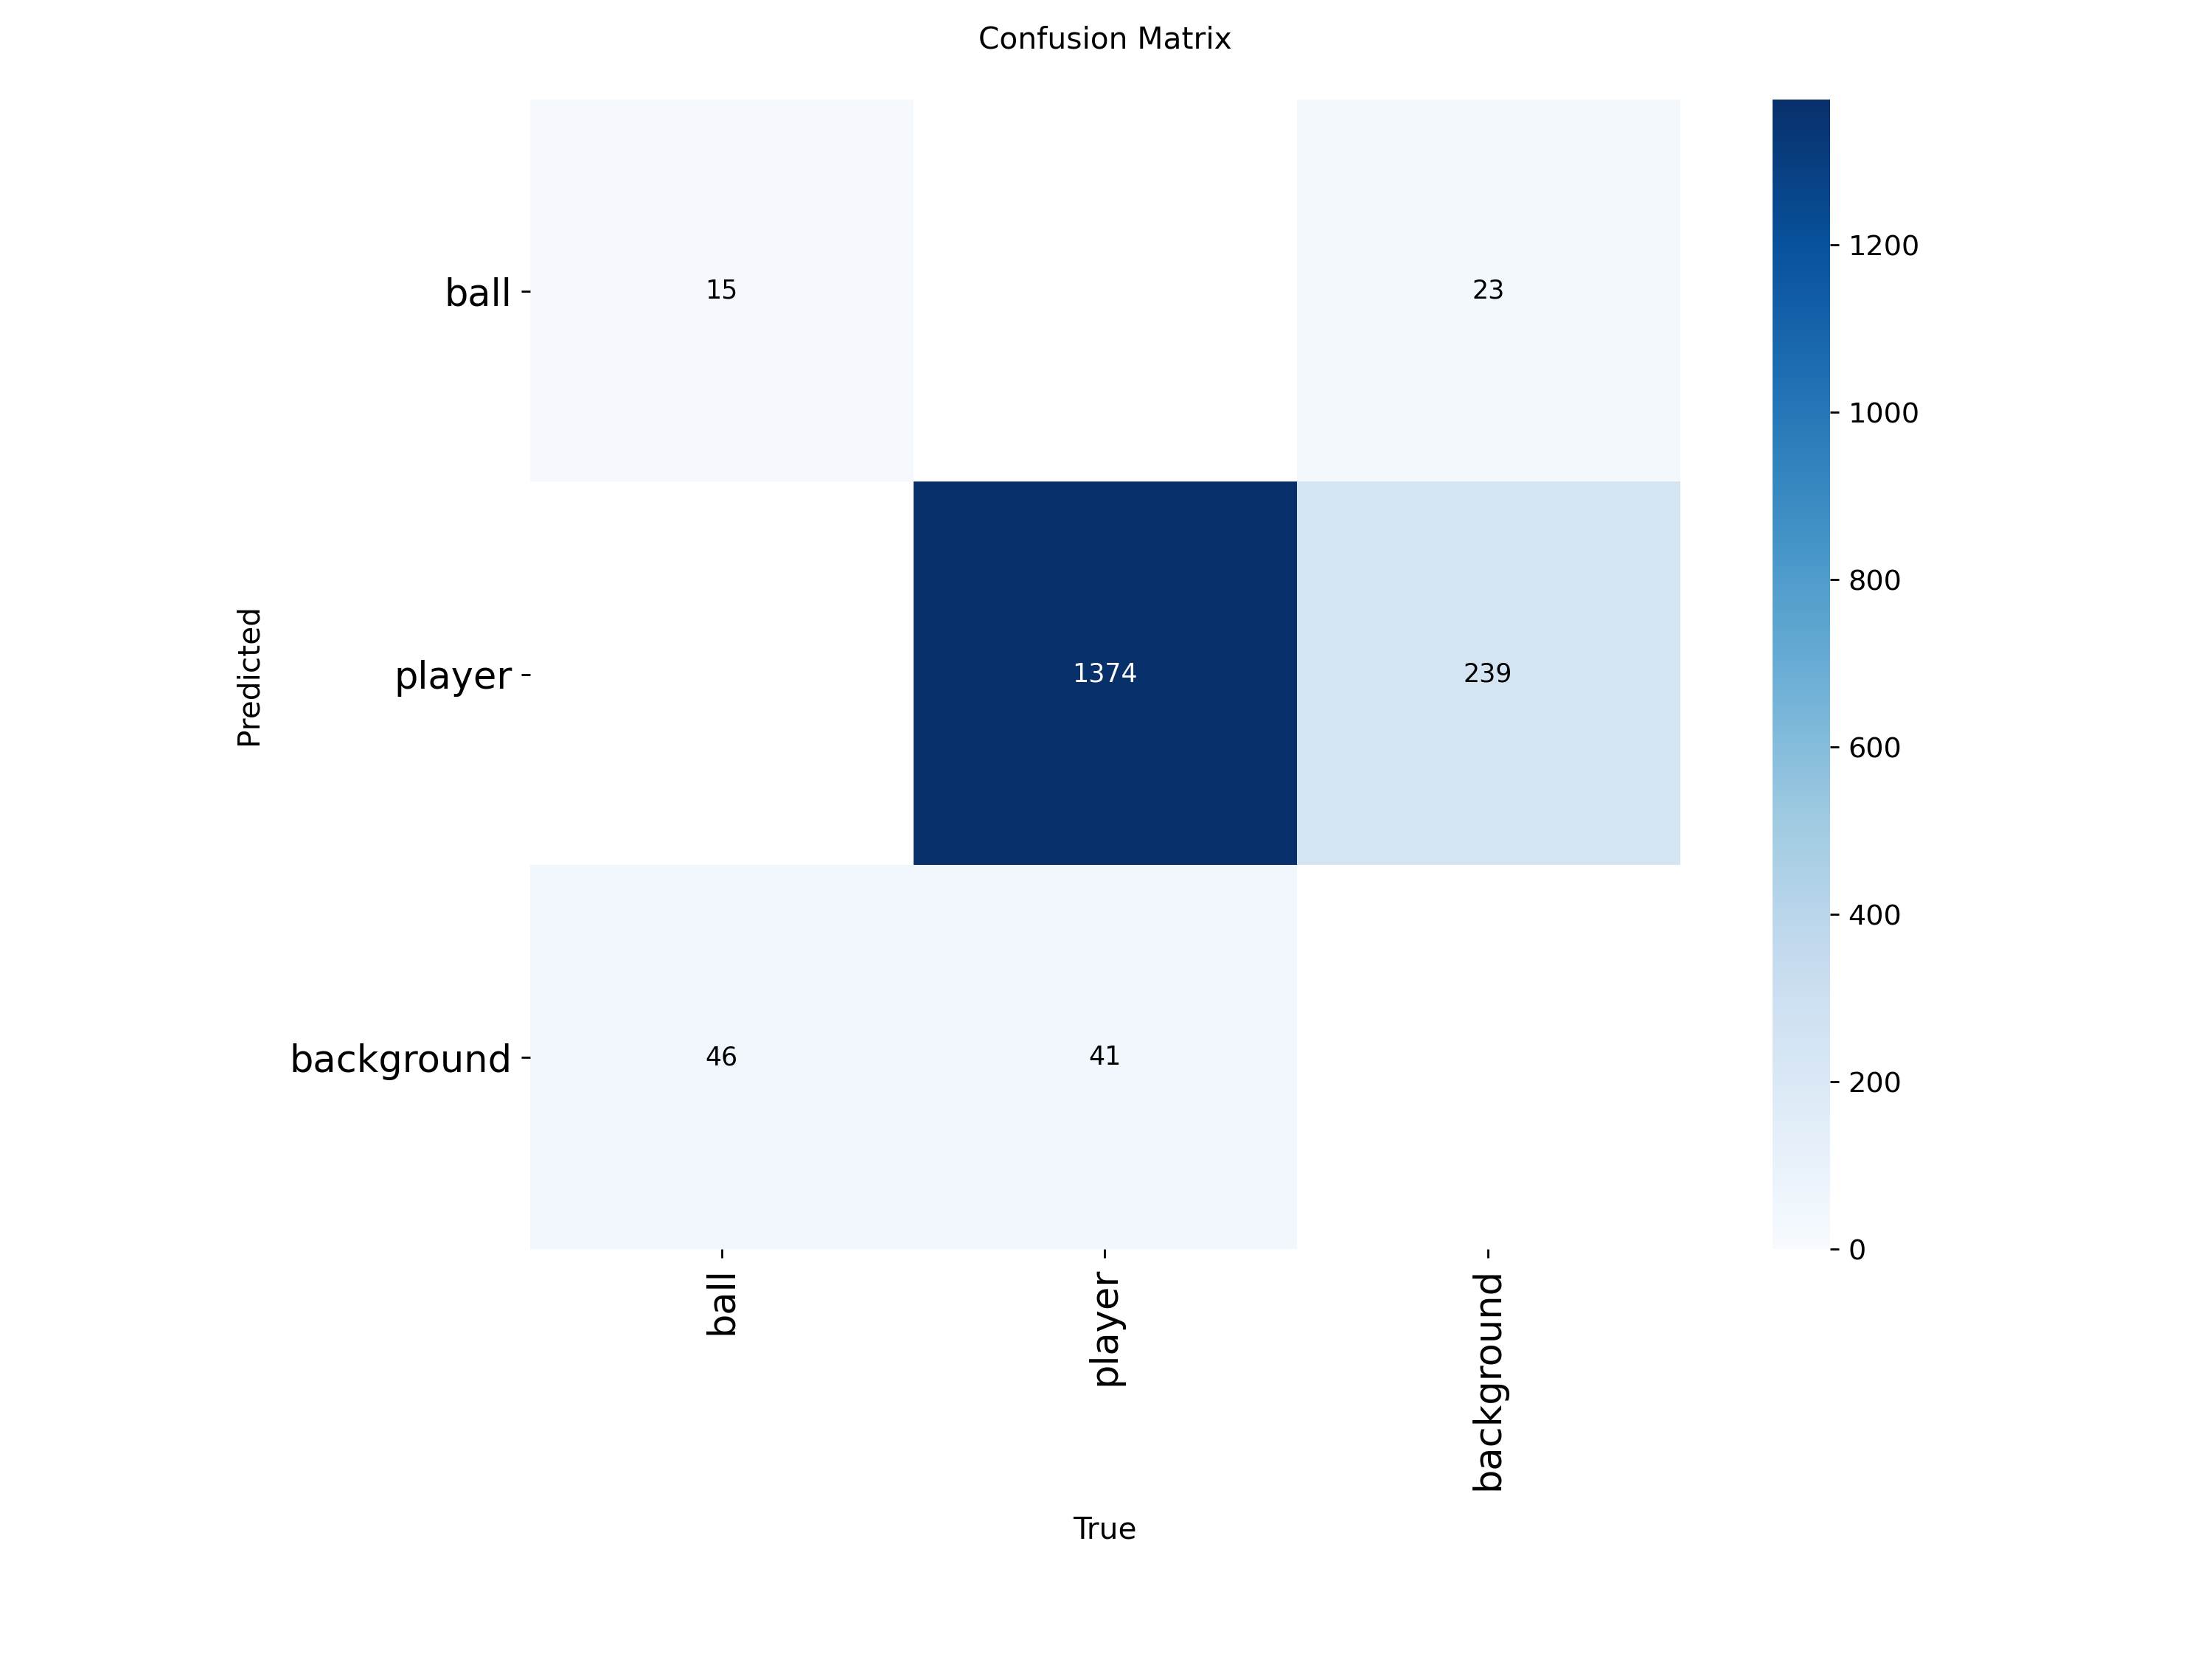
\includegraphics[width=0.8\textwidth]{figures/confusion_matrix_m.png}
    \caption{Confusion matrix for the YOLOv8m model}
    \label{fig:cm_m}
\end{figure}

\subsection{Training Summary}
The training results demonstrate a very clear picture of the accuracy of each model, as well as their shortcomings. Player detection is very strong across all three variants, with each of them achieving mAP@0.5 scores of over 0.9 on that class. However, as previous studies investigated in our literature review section of this thesis, ball detection remains a challenge, with none of the models achieving mAP@0.5 scores over 0.3. This indicates the dataset size and image resolution as constraints, as there are not enough instances of the ball class and the ball being a small object gets confused with the background due to the small number of pixels.

\section{Inference Benchmarks}
This section will present the inference benchmark results for all three YOLOv8 variants, in each of our hardware configurations as described in the methodology chapter of this thesis. The inference test video is the same for all: a 1920x1080 video which is 15 seconds long with 30 FPS. This gives us a total of 750 frames, which get resized to 640x640 to fit in our pipeline. 

\subsection{Device A – Discrete NVIDIA GeForce RTX 3060 12GB GPU (CUDA)}
On Device A the three models deliver markedly different throughput. Interestingly the nano variant performed very slightly slower than the small, but that can be attributed to warmups as the nano inference was run first. On equal conditions, the nano variant should be expected to perform faster. Another significant gap is between the small and medium variants, as we notice a drop of 33\% in FPS going from YOLOv8s to YOLOv8m. 

\begin{table}[H]
\centering
\small
\label{tab:inference_rtx3060_summary}
\begin{tabular}{lrrrrrr}
\toprule
\textbf{Model} & \textbf{Total dets.} & \textbf{Dets/frame} & \textbf{Mean conf.} & \textbf{Med. conf.} & \textbf{Std conf.} & \textbf{Inference FPS} \\
\midrule
YOLOv8n & 15{,}518 & 20.69 & 0.503 & 0.520 & 0.109 & 78.3 \\
YOLOv8s & 17{,}114 & 22.82 & 0.563 & 0.591 & 0.119 & 82.3 \\
YOLOv8m & 16{,}686 & 22.25 & 0.578 & 0.609 & 0.111 & 55.1 \\
\bottomrule
\end{tabular}
\caption{Inference summary statistics for all three YOLOv8 variants on Device A (RTX 3060, CUDA).}
\end{table}

Related to the overall performance of the models, all of them comfortably exceed the 25 FPS threshold commonly considered the minimum for smooth real-time video. This shows that a machine fitted with a discrete GPU should have no problem on object detection from video, and in fact may even be encouraged to try the larger YOLOv8l(large) model.

\subsection{Detection Volume and Confidence}
YOLOv8s produces the highest total detection count at 17,114 detections across 750 frames (22.82 detections per frame on average), compared to 16,686 for YOLOv8m and 15,518 for YOLOv8n. Importantly, no frame across any of the three models returned zero detections, indicating consistent coverage of the video content under the selected confidence threshold.

The confidence statistics reveal a clear ordering with model scale. Mean confidence increases from 0.503 (YOLOv8n) to 0.563 (YOLOv8s) to 0.578 (YOLOv8m), as does median confidence. This pattern reflects the expected relationship between model capacity and calibration.

The per-class breakdown in Table 4.4 reinforces the class-level findings from the training evaluation. Player detections dominate the detection volume across all three models, accounting for between 95.8\% and 97.9\% of all detections. Ball detections remain a small fraction of the total in all cases, consistent with the low ball AP scores reported in Section 4.1.3.

\begin{table}[h]
\centering
\label{tab:inference_rtx3060_class}
\begin{tabular}{lrrrrr}
\toprule
\textbf{Model} & \textbf{Dets [ball]} & \textbf{Dets [player]} & \textbf{Ball \%} & \textbf{Player \%} & \textbf{Mean conf.} \\
\midrule
YOLOv8n & 319 & 15{,}199 & 2.1\% & 97.9\% & 0.503 \\
YOLOv8s & 717 & 16{,}397 & 4.2\% & 95.8\% & 0.563 \\
YOLOv8m & 529 & 16{,}157 & 3.2\% & 96.8\% & 0.578 \\
\bottomrule
\end{tabular}
\caption{Per-class detection counts and proportions for all three YOLOv8 variants on Device A (RTX 3060, CUDA).}
\end{table}

Table 4.5 and the subsequent Figure 4.8 present the full confidence score distribution across all detections for each model. The distributions show a clear shift toward higher confidence bins as model capacity increases. YOLOv8n is heavily concentrated in the 0.40–0.60 range, with its modal bin at 0.50–0.60 (5,583 detections) and only 86 detections above 0.70. YOLOv8s and YOLOv8m both show a marked redistribution of detections into the 0.60–0.70 bin, which becomes the modal bin for both models (6,638 and 7,833 detections respectively), with YOLOv8s also contributing 1,381 detections in the 0.70–0.80 range. No detections from any model exceed 0.80, which reflects the inherent difficulty of the task, particularly for ball detection, and is consistent with the moderate mAP@0.5 scores reported during training.

\begin{table}[h]
\centering
\label{tab:inference_rtx3060_conf_dist}
\begin{tabular}{lrrr}
\toprule
\textbf{Confidence bin} & \textbf{YOLOv8n} & \textbf{YOLOv8s} & \textbf{YOLOv8m} \\
\midrule
0.25 -- 0.30 & 801   & 689   & 520   \\
0.30 -- 0.40 & 2{,}247 & 1{,}462 & 1{,}125 \\
0.40 -- 0.50 & 3{,}680 & 2{,}253 & 1{,}824 \\
0.50 -- 0.60 & 5{,}583 & 4{,}691 & 4{,}299 \\
0.60 -- 0.70 & 3{,}121 & 6{,}638 & 7{,}833 \\
0.70 -- 0.80 & 86    & 1{,}381 & 1{,}085 \\
0.80 -- 0.90 & 0     & 0     & 0     \\
0.90 -- 1.00 & 0     & 0     & 0     \\
\bottomrule
\end{tabular}
\caption{Confidence score distribution across bins for all three YOLOv8 variants on Device A (RTX 3060, CUDA).}
\end{table}

\begin{figure}[H]
    \centering
    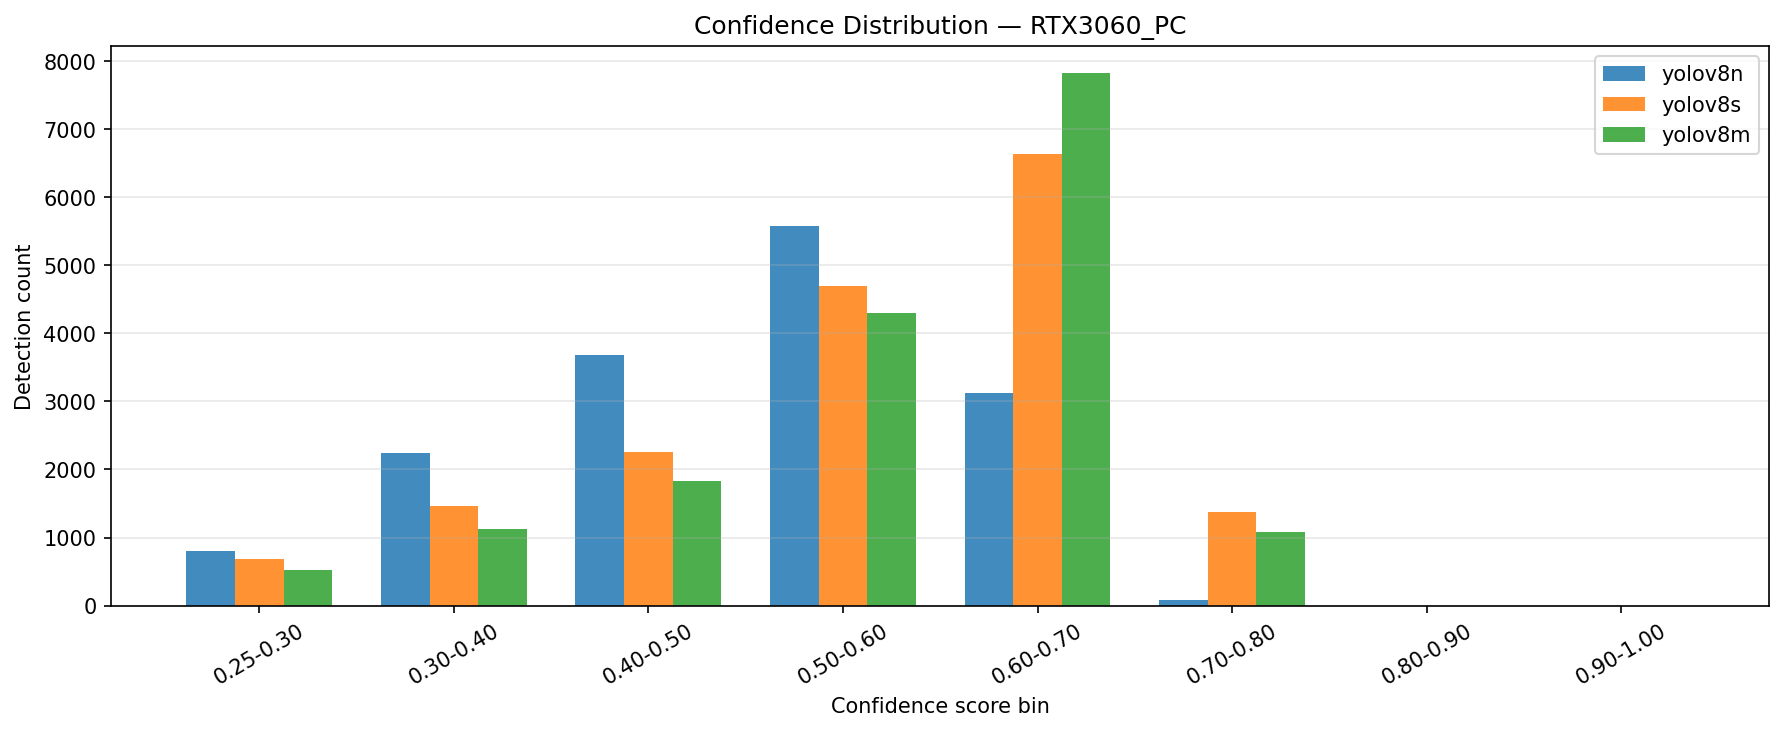
\includegraphics[width=1\textwidth]{figures/inference_RTX3060_PC_conf_distribution.png}
    \caption{Confidence distribution for all models on Device A(RTX 3060, CUDA).}
    \label{fig:confidence_3060}
\end{figure}

\subsection{Device B – Apple MacBook Pro M4 (MPS)}
On Device B the three models show a noticeably different speed profile compared to Device A. YOLOv8n and YOLOv8s run at nearly identical throughput of 57.1 and 56.5 FPS respectively, a gap of only 1.1\% that is not practically meaningful. The medium variant drops more sharply to 34.6 FPS, a reduction of 38.8\% relative to YOLOv8s. Compared to Device A, all three models are slower: YOLOv8n loses 27.1\% of its RTX 3060 throughput, YOLOv8s loses 31.3\%, and YOLOv8m loses 37.2\%, indicating that the performance gap widens with model size on this hardware. Despite this, all three variants remain well above the 25 FPS threshold considered the minimum for smooth real-time video processing.

\begin{table}[h]
\centering
\label{tab:inference_m4_summary}
\resizebox{\textwidth}{!}{%
\begin{tabular}{lrrrrrr}
\toprule
\textbf{Model} & \textbf{Total dets.} & \textbf{Dets/frame} & \textbf{Mean conf.} & \textbf{Med. conf.} & \textbf{Std conf.} & \textbf{Inference FPS} \\
\midrule
YOLOv8n & 15{,}526 & 20.70 & 0.503 & 0.520 & 0.109 & 57.1 \\
YOLOv8s & 17{,}094 & 22.79 & 0.564 & 0.591 & 0.119 & 56.5 \\
YOLOv8m & 16{,}691 & 22.25 & 0.577 & 0.609 & 0.111 & 34.6 \\
\bottomrule
\end{tabular}%
}
\caption{Inference summary statistics for all three YOLOv8 variants on Device B (Apple M4, MPS).}
\end{table}

The detection counts on Device B are virtually identical to those recorded on Device A, which is expected given that the same model weights and inference settings were used across both devices. YOLOv8s again produces the highest total at 17,094 detections (22.79 per frame), followed by YOLOv8m at 16,691 and YOLOv8n at 15,526. No frame returned zero detections across any model, confirming consistent coverage. The confidence statistics are likewise stable: mean confidence follows the same ordering of 0.503 (YOLOv8n), 0.564 (YOLOv8s), and 0.577 (YOLOv8m), reinforcing that the MPS backend introduces no meaningful change in detection quality relative to CUDA.

The per-class breakdown in Table 4.7 again shows player detections predominantly between 95.8\% and 97.9\% of total detections. Ball detection counts closely mirror the Device A results, with YOLOv8s producing the highest ball count at 716, followed by YOLOv8m at 529 and YOLOv8n at 322, preserving the same non-linear ordering observed during training.

\begin{table}[H]
\centering
\label{tab:inference_m4_class}
\begin{tabular}{lrrrrr}
\toprule
\textbf{Model} & \textbf{Dets [ball]} & \textbf{Dets [player]} & \textbf{Ball \%} & \textbf{Player \%} & \textbf{Mean conf.} \\
\midrule
YOLOv8n & 322 & 15{,}204 & 2.1\% & 97.9\% & 0.503 \\
YOLOv8s & 716 & 16{,}378 & 4.2\% & 95.8\% & 0.564 \\
YOLOv8m & 529 & 16{,}162 & 3.2\% & 96.8\% & 0.577 \\
\bottomrule
\end{tabular}
\caption{Per-class detection counts and proportions for all three YOLOv8 variants on Device B (Apple M4, MPS).}
\end{table}

Table 4.8 and Figure 4.9 present the confidence score distribution across all detections on Device B. The pattern is near-identical to that observed on Device A, which again confirms that backend differences between CUDA and MPS do not affect detection quality. YOLOv8n remains concentrated in the 0.40–0.60 range, with its modal bin at 0.50–0.60 (5,581 detections) and only 85 detections above 0.70. YOLOv8s and YOLOv8m again shift their modal bin to 0.60–0.70 (6,660 and 7,831 detections respectively), and YOLOv8s contributes 1,382 detections in the 0.70–0.80 range. As on Device A, no detections from any model exceed 0.80.

\begin{table}[H]
\centering
\label{tab:inference_m4_conf_dist}
\begin{tabular}{lrrr}
\toprule
\textbf{Confidence bin} & \textbf{YOLOv8n} & \textbf{YOLOv8s} & \textbf{YOLOv8m} \\
\midrule
0.25 -- 0.30 & 799   & 673   & 535   \\
0.30 -- 0.40 & 2{,}235 & 1{,}474 & 1{,}121 \\
0.40 -- 0.50 & 3{,}710 & 2{,}254 & 1{,}792 \\
0.50 -- 0.60 & 5{,}581 & 4{,}651 & 4{,}343 \\
0.60 -- 0.70 & 3{,}116 & 6{,}660 & 7{,}831 \\
0.70 -- 0.80 & 85    & 1{,}382 & 1{,}069 \\
0.80 -- 0.90 & 0     & 0     & 0     \\
0.90 -- 1.00 & 0     & 0     & 0     \\
\bottomrule
\end{tabular}
\caption{Confidence score distribution across bins for all three YOLOv8 variants on Device B (Apple M4, MPS).}
\end{table}

\begin{figure}[H]
    \centering
    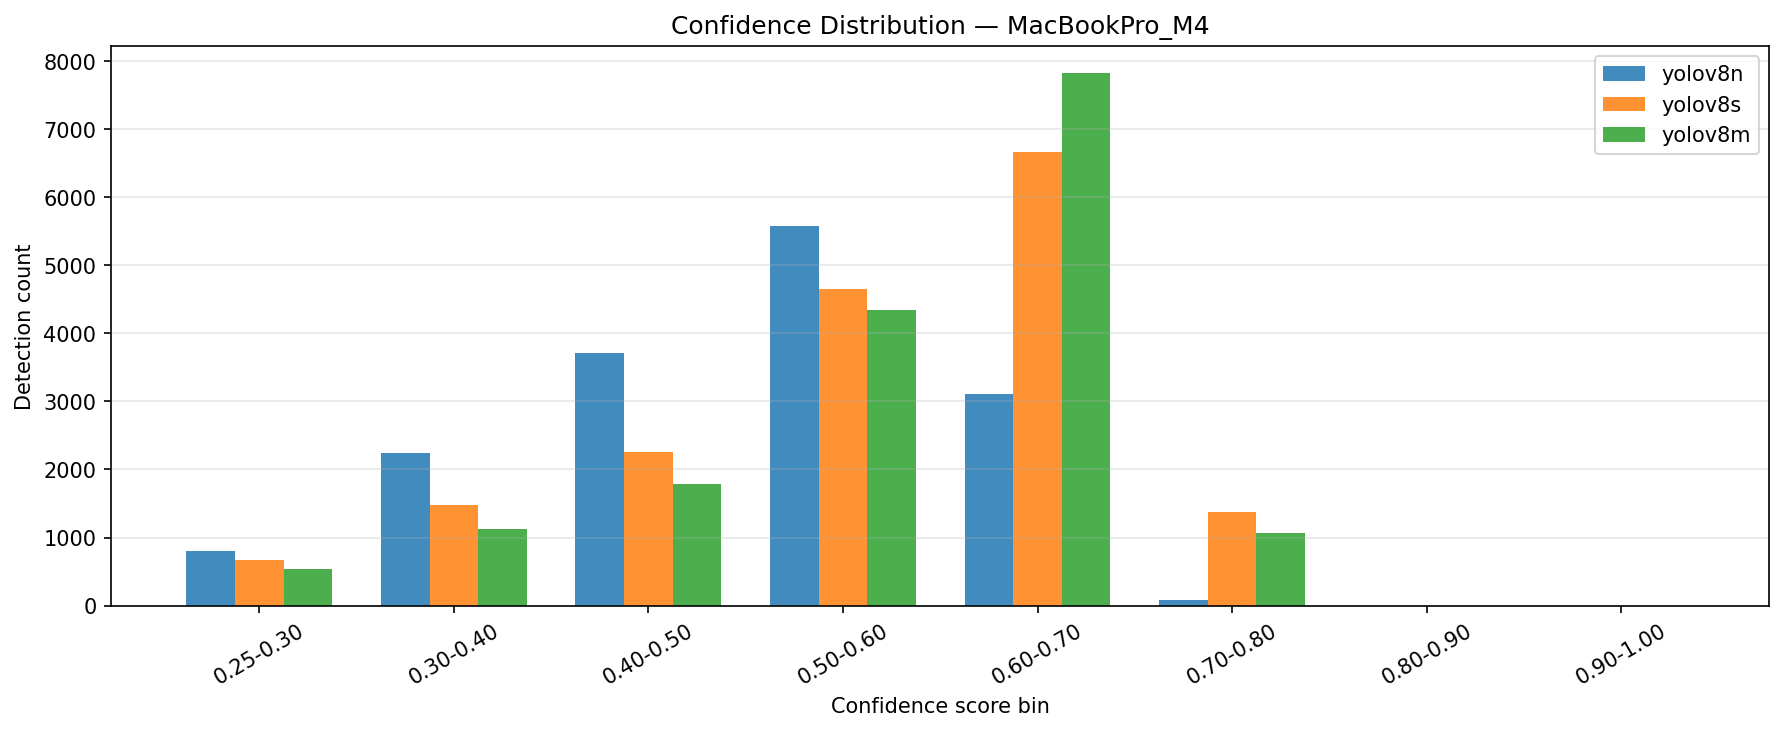
\includegraphics[width=1\textwidth]{figures/inference_MacBookPro_M4_conf_distribution.png}
    \caption{Confidence distribution for all models on Device B(MacBook Pro M4, MPS).}
    \label{fig:confidence_MB}
\end{figure}

\subsection{Device C – Lenovo ThinkPad T490s (CPU only)}
Device C presents the most difficult environment out of the three in our testing. Due to the lack of a GPU, inference is run entirely on the Intel Core i7-8665U CPU with no hardware acceleration. As a consequence of this, the impact on performance is dramatic. Only the nano model reaches double digits in FPS figures at 14.1 FPS, while the others are far below (YOLOv8s – 6.6 FPS, YOLOv8m – 2.9 FPS). As none of the models passes the 25 FPS threshold, Device C proves incapable of providing smooth real-time object detection, even on the lightest and most inaccurate model. This, however, does not mean it does not have its uses, as we will discuss in latter sections of our thesis.

\begin{table}[H]
\centering

\label{tab:inference_cpu_summary}
\resizebox{\textwidth}{!}{%
\begin{tabular}{lrrrrrr}
\toprule
\textbf{Model} & \textbf{Total dets.} & \textbf{Dets/frame} & \textbf{Mean conf.} & \textbf{Med. conf.} & \textbf{Std conf.} & \textbf{Inference FPS} \\
\midrule
YOLOv8n & 15{,}518 & 20.69 & 0.503 & 0.520 & 0.109 & 14.1 \\
YOLOv8s & 17{,}110 & 22.81 & 0.563 & 0.591 & 0.119 &  6.6 \\
YOLOv8m & 16{,}687 & 22.25 & 0.578 & 0.609 & 0.111 &  2.9 \\
\bottomrule
\end{tabular}%
}
\caption{Inference summary statistics for all three YOLOv8 variants on Device C (Lenovo ThinkPad T490s, CPU only).}
\end{table}

The per-class breakdown in Table 4.10 again shows the same pattern seen across all devices. Player detections account for the overwhelming majority of all detections, as is to be expected. Ball detection counts are identical to those on Device A, with YOLOv8s producing 717 ball detections, YOLOv8m producing 529, and YOLOv8n producing 319, preserving the non-monotonic ordering established in training across all three hardware configurations.
\begin{table}[H]
\centering
\caption{Per-class detection counts and proportions for all three YOLOv8 variants on Device C (Lenovo ThinkPad T490s, CPU only).}
\label{tab:inference_cpu_class}
\begin{tabular}{lrrrrr}
\toprule
\textbf{Model} & \textbf{Dets [ball]} & \textbf{Dets [player]} & \textbf{Ball \%} & \textbf{Player \%} & \textbf{Mean conf.} \\
\midrule
YOLOv8n & 319 & 15{,}199 & 2.1\% & 97.9\% & 0.503 \\
YOLOv8s & 717 & 16{,}393 & 4.2\% & 95.8\% & 0.563 \\
YOLOv8m & 529 & 16{,}158 & 3.2\% & 96.8\% & 0.578 \\
\bottomrule
\end{tabular}
\end{table}
Table 4.11 presents the confidence score distribution on Device C. The distributions are near-identical to those recorded on Devices A and B, providing the strongest confirmation yet that the choice of hardware backend, be it CUDA, MPS, or CPU, has no effect on detection confidence. YOLOv8n remains concentrated in the 0.40--0.60 range, with its modal bin at 0.50--0.60 (5,583 detections) and only 86 detections above 0.70. YOLOv8s and YOLOv8m again shift their modal bin to 0.60--0.70 (6,635 and 7,836 detections respectively), with YOLOv8s contributing 1,384 detections in the 0.70--0.80 range. No detections from any model exceed 0.80.

\begin{table}[H]
\centering
\label{tab:inference_cpu_conf_dist}
\begin{tabular}{lrrr}
\toprule
\textbf{Confidence bin} & \textbf{YOLOv8n} & \textbf{YOLOv8s} & \textbf{YOLOv8m} \\
\midrule
0.25 -- 0.30 & 800   & 685   & 520   \\
0.30 -- 0.40 & 2{,}247 & 1{,}462 & 1{,}128 \\
0.40 -- 0.50 & 3{,}679 & 2{,}251 & 1{,}821 \\
0.50 -- 0.60 & 5{,}583 & 4{,}693 & 4{,}297 \\
0.60 -- 0.70 & 3{,}123 & 6{,}635 & 7{,}836 \\
0.70 -- 0.80 & 86    & 1{,}384 & 1{,}085 \\
0.80 -- 0.90 & 0     & 0     & 0     \\
0.90 -- 1.00 & 0     & 0     & 0     \\
\bottomrule
\end{tabular}
\caption{Confidence score distribution across bins for all three YOLOv8 variants on Device C (Lenovo ThinkPad T490s, CPU only).}
\end{table}

\begin{figure}[H]
    \centering
    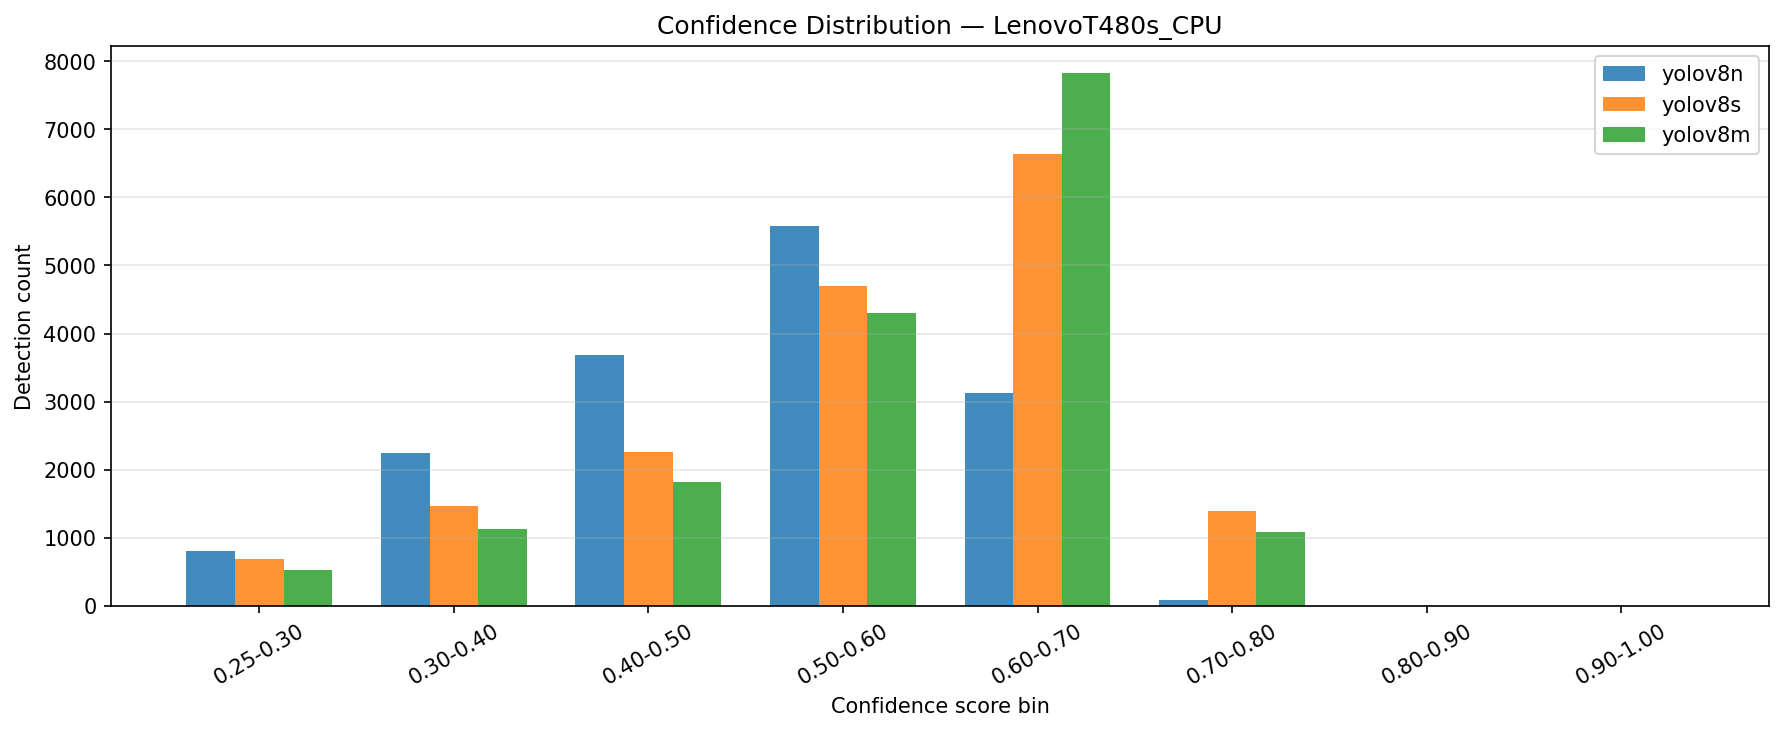
\includegraphics[width=1\textwidth]{figures/inference_LenovoT480s_CPU_conf_distribution.png}
    \caption{Confidence distribution for all models on Device C(Lenovo Thinkpad T490s, CPU).}
    \label{fig:confidence_TP}
\end{figure}

\section{Summary}
This chapter presented the results of the training and inference experiments across all three YOLOv8 variants and the three consumer-grade hardware configurations. The training evaluation established a clear accuracy hierarchy: YOLOv8m achieves the highest overall mAP@0.5 at 0.617, followed closely by YOLOv8s at 0.613, while YOLOv8n trails noticeably at 0.534. Player detection is strong across all three models, with each exceeding an AP of 0.90 on that class. Ball detection remains the persistent challenge of the domain, with no model surpassing an AP of 0.27, a limitation attributed to the small spatial footprint of the ball at 640×640 resolution and the limited number of ball instances in the dataset. Notably, YOLOv8s outperforms YOLOv8m on ball detection despite being the smaller model, a non-linear result explained by the medium model's tendency to overfit to the underrepresented ball class.

The inference benchmarks reveal that hardware selection has a decisive impact on throughput but no effect on detection quality, as confidence distributions and detection counts were consistent across all three devices. On Device A, all three models run at real-time speeds under CUDA, with YOLOv8n and YOLOv8s both exceeding 78 FPS and YOLOv8m reaching 55 FPS. Device B delivers moderate throughput under MPS, with YOLOv8n and YOLOv8s both near 57 FPS and YOLOv8m at 34.6 FPS, all above the 25 FPS real-time threshold. Device C exposes the severe cost of CPU-only inference: only YOLOv8n reaches 14.1 FPS, while YOLOv8s and YOLOv8m fall to 6.6 and 2.9 FPS respectively, making them unsuitable for real-time deployment on this hardware tier.